% Options for packages loaded elsewhere
\PassOptionsToPackage{unicode}{hyperref}
\PassOptionsToPackage{hyphens}{url}
%
\documentclass[
]{book}
\title{Perbandingan Smoothing, ARIMA, dan ARIMAX untuk prediksi harga minyak mentah}
\author{Adley Dityo Valentinus Putra (G14180009) \and Muhammad Ammar Sahab (G14190020) \and Putri Eka Perdanti (G14190027) \and Farhan Narendra Achyara (G14190050) \and Grashella Clara Nesa Br Ginting (G14190086)}
\date{2022-04-10}

\usepackage{amsmath,amssymb}
\usepackage{lmodern}
\usepackage{iftex}
\ifPDFTeX
  \usepackage[T1]{fontenc}
  \usepackage[utf8]{inputenc}
  \usepackage{textcomp} % provide euro and other symbols
\else % if luatex or xetex
  \usepackage{unicode-math}
  \defaultfontfeatures{Scale=MatchLowercase}
  \defaultfontfeatures[\rmfamily]{Ligatures=TeX,Scale=1}
\fi
% Use upquote if available, for straight quotes in verbatim environments
\IfFileExists{upquote.sty}{\usepackage{upquote}}{}
\IfFileExists{microtype.sty}{% use microtype if available
  \usepackage[]{microtype}
  \UseMicrotypeSet[protrusion]{basicmath} % disable protrusion for tt fonts
}{}
\makeatletter
\@ifundefined{KOMAClassName}{% if non-KOMA class
  \IfFileExists{parskip.sty}{%
    \usepackage{parskip}
  }{% else
    \setlength{\parindent}{0pt}
    \setlength{\parskip}{6pt plus 2pt minus 1pt}}
}{% if KOMA class
  \KOMAoptions{parskip=half}}
\makeatother
\usepackage{xcolor}
\IfFileExists{xurl.sty}{\usepackage{xurl}}{} % add URL line breaks if available
\IfFileExists{bookmark.sty}{\usepackage{bookmark}}{\usepackage{hyperref}}
\hypersetup{
  pdftitle={Perbandingan Smoothing, ARIMA, dan ARIMAX untuk prediksi harga minyak mentah},
  pdfauthor={Adley Dityo Valentinus Putra (G14180009); Muhammad Ammar Sahab (G14190020); Putri Eka Perdanti (G14190027); Farhan Narendra Achyara (G14190050); Grashella Clara Nesa Br Ginting (G14190086)},
  hidelinks,
  pdfcreator={LaTeX via pandoc}}
\urlstyle{same} % disable monospaced font for URLs
\usepackage{color}
\usepackage{fancyvrb}
\newcommand{\VerbBar}{|}
\newcommand{\VERB}{\Verb[commandchars=\\\{\}]}
\DefineVerbatimEnvironment{Highlighting}{Verbatim}{commandchars=\\\{\}}
% Add ',fontsize=\small' for more characters per line
\usepackage{framed}
\definecolor{shadecolor}{RGB}{248,248,248}
\newenvironment{Shaded}{\begin{snugshade}}{\end{snugshade}}
\newcommand{\AlertTok}[1]{\textcolor[rgb]{0.94,0.16,0.16}{#1}}
\newcommand{\AnnotationTok}[1]{\textcolor[rgb]{0.56,0.35,0.01}{\textbf{\textit{#1}}}}
\newcommand{\AttributeTok}[1]{\textcolor[rgb]{0.77,0.63,0.00}{#1}}
\newcommand{\BaseNTok}[1]{\textcolor[rgb]{0.00,0.00,0.81}{#1}}
\newcommand{\BuiltInTok}[1]{#1}
\newcommand{\CharTok}[1]{\textcolor[rgb]{0.31,0.60,0.02}{#1}}
\newcommand{\CommentTok}[1]{\textcolor[rgb]{0.56,0.35,0.01}{\textit{#1}}}
\newcommand{\CommentVarTok}[1]{\textcolor[rgb]{0.56,0.35,0.01}{\textbf{\textit{#1}}}}
\newcommand{\ConstantTok}[1]{\textcolor[rgb]{0.00,0.00,0.00}{#1}}
\newcommand{\ControlFlowTok}[1]{\textcolor[rgb]{0.13,0.29,0.53}{\textbf{#1}}}
\newcommand{\DataTypeTok}[1]{\textcolor[rgb]{0.13,0.29,0.53}{#1}}
\newcommand{\DecValTok}[1]{\textcolor[rgb]{0.00,0.00,0.81}{#1}}
\newcommand{\DocumentationTok}[1]{\textcolor[rgb]{0.56,0.35,0.01}{\textbf{\textit{#1}}}}
\newcommand{\ErrorTok}[1]{\textcolor[rgb]{0.64,0.00,0.00}{\textbf{#1}}}
\newcommand{\ExtensionTok}[1]{#1}
\newcommand{\FloatTok}[1]{\textcolor[rgb]{0.00,0.00,0.81}{#1}}
\newcommand{\FunctionTok}[1]{\textcolor[rgb]{0.00,0.00,0.00}{#1}}
\newcommand{\ImportTok}[1]{#1}
\newcommand{\InformationTok}[1]{\textcolor[rgb]{0.56,0.35,0.01}{\textbf{\textit{#1}}}}
\newcommand{\KeywordTok}[1]{\textcolor[rgb]{0.13,0.29,0.53}{\textbf{#1}}}
\newcommand{\NormalTok}[1]{#1}
\newcommand{\OperatorTok}[1]{\textcolor[rgb]{0.81,0.36,0.00}{\textbf{#1}}}
\newcommand{\OtherTok}[1]{\textcolor[rgb]{0.56,0.35,0.01}{#1}}
\newcommand{\PreprocessorTok}[1]{\textcolor[rgb]{0.56,0.35,0.01}{\textit{#1}}}
\newcommand{\RegionMarkerTok}[1]{#1}
\newcommand{\SpecialCharTok}[1]{\textcolor[rgb]{0.00,0.00,0.00}{#1}}
\newcommand{\SpecialStringTok}[1]{\textcolor[rgb]{0.31,0.60,0.02}{#1}}
\newcommand{\StringTok}[1]{\textcolor[rgb]{0.31,0.60,0.02}{#1}}
\newcommand{\VariableTok}[1]{\textcolor[rgb]{0.00,0.00,0.00}{#1}}
\newcommand{\VerbatimStringTok}[1]{\textcolor[rgb]{0.31,0.60,0.02}{#1}}
\newcommand{\WarningTok}[1]{\textcolor[rgb]{0.56,0.35,0.01}{\textbf{\textit{#1}}}}
\usepackage{longtable,booktabs,array}
\usepackage{calc} % for calculating minipage widths
% Correct order of tables after \paragraph or \subparagraph
\usepackage{etoolbox}
\makeatletter
\patchcmd\longtable{\par}{\if@noskipsec\mbox{}\fi\par}{}{}
\makeatother
% Allow footnotes in longtable head/foot
\IfFileExists{footnotehyper.sty}{\usepackage{footnotehyper}}{\usepackage{footnote}}
\makesavenoteenv{longtable}
\usepackage{graphicx}
\makeatletter
\def\maxwidth{\ifdim\Gin@nat@width>\linewidth\linewidth\else\Gin@nat@width\fi}
\def\maxheight{\ifdim\Gin@nat@height>\textheight\textheight\else\Gin@nat@height\fi}
\makeatother
% Scale images if necessary, so that they will not overflow the page
% margins by default, and it is still possible to overwrite the defaults
% using explicit options in \includegraphics[width, height, ...]{}
\setkeys{Gin}{width=\maxwidth,height=\maxheight,keepaspectratio}
% Set default figure placement to htbp
\makeatletter
\def\fps@figure{htbp}
\makeatother
\setlength{\emergencystretch}{3em} % prevent overfull lines
\providecommand{\tightlist}{%
  \setlength{\itemsep}{0pt}\setlength{\parskip}{0pt}}
\setcounter{secnumdepth}{5}
\newlength{\cslhangindent}
\setlength{\cslhangindent}{1.5em}
\newlength{\csllabelwidth}
\setlength{\csllabelwidth}{3em}
\newlength{\cslentryspacingunit} % times entry-spacing
\setlength{\cslentryspacingunit}{\parskip}
\newenvironment{CSLReferences}[2] % #1 hanging-ident, #2 entry spacing
 {% don't indent paragraphs
  \setlength{\parindent}{0pt}
  % turn on hanging indent if param 1 is 1
  \ifodd #1
  \let\oldpar\par
  \def\par{\hangindent=\cslhangindent\oldpar}
  \fi
  % set entry spacing
  \setlength{\parskip}{#2\cslentryspacingunit}
 }%
 {}
\usepackage{calc}
\newcommand{\CSLBlock}[1]{#1\hfill\break}
\newcommand{\CSLLeftMargin}[1]{\parbox[t]{\csllabelwidth}{#1}}
\newcommand{\CSLRightInline}[1]{\parbox[t]{\linewidth - \csllabelwidth}{#1}\break}
\newcommand{\CSLIndent}[1]{\hspace{\cslhangindent}#1}
\usepackage{booktabs}
\ifLuaTeX
  \usepackage{selnolig}  % disable illegal ligatures
\fi

\begin{document}
\maketitle

{
\setcounter{tocdepth}{1}
\tableofcontents
}
\hypertarget{pendahuluan}{%
\chapter*{Pendahuluan}\label{pendahuluan}}
\addcontentsline{toc}{chapter}{Pendahuluan}

\url{https://bookdown.org/mammarsahab3/LaporanMPDW/}

\hypertarget{struktur-penelitian}{%
\section*{Struktur penelitian}\label{struktur-penelitian}}
\addcontentsline{toc}{section}{Struktur penelitian}

Laporan ini akan membandingkan beberapa metode peralaman deret waktu untuk data harga minyak mentah. Metode tersebut akan dilatih menggunakan harga minyak mentah dari tahun 2009 sampai 2016, lalu diuji dengan meramal harga minyak mentah tahun 2017. Pembagian tersebut juga dilakukan di (\protect\hyperlink{ref-He2018}{He 2018}), yang membandingkan model deret waktu seperti pemulusan dan ARIMA dengan model pembelajaran mesin (SVM). Berbeda dengan penelitian tersebut, penelitian ini akan menambahkan jenis pemulusan yang dipakai, serta mencoba menambahkan pengaruh peubah bebas \emph{dummy} yang memodelkan efek hari setelah libur, peubahan struktural pada rezim harga minyak, dan lain-lain. Sekarang, penulisan laporan masih dalam tahap praproses dan eksplorasi data.

\hypertarget{ekstraksi-data}{%
\section*{Ekstraksi data}\label{ekstraksi-data}}
\addcontentsline{toc}{section}{Ekstraksi data}

Dataset yang digunakan sebagai berikut. Ambil data minyak dari tahun 2000 sampai sekarang \texttt{Sys.Date()} dengam bantuan library \texttt{quantmod} (\protect\hyperlink{ref-R-quantmod}{Ryan dan Ulrich 2020}):

\begin{Shaded}
\begin{Highlighting}[]
\FunctionTok{library}\NormalTok{(quantmod)}
\FunctionTok{library}\NormalTok{(dtplyr)}
\FunctionTok{library}\NormalTok{(dplyr)}

\NormalTok{start }\OtherTok{\textless{}{-}} \FunctionTok{as.POSIXct}\NormalTok{(}\StringTok{"2000{-}08{-}23"}\NormalTok{)}
\NormalTok{end }\OtherTok{\textless{}{-}} \FunctionTok{as.POSIXct}\NormalTok{(}\FunctionTok{Sys.Date}\NormalTok{())}

\FunctionTok{getSymbols}\NormalTok{(}\AttributeTok{Symbols =} \StringTok{"CL=F"}\NormalTok{,}\AttributeTok{src =} \StringTok{"yahoo"}\NormalTok{, }\AttributeTok{from =}\NormalTok{ start, }\AttributeTok{to =}\NormalTok{ end)}

\NormalTok{crude}\OtherTok{\textless{}{-}} \FunctionTok{lazy\_dt}\NormalTok{(}\StringTok{\textasciigrave{}}\AttributeTok{CL=F}\StringTok{\textasciigrave{}}\NormalTok{) }\SpecialCharTok{\%\textgreater{}\%} 
  \FunctionTok{mutate}\NormalTok{(}\AttributeTok{X=}\FunctionTok{as.Date}\NormalTok{(index,}\AttributeTok{format=}\StringTok{"\%d/\%m/\%Y"}\NormalTok{)) }\SpecialCharTok{\%\textgreater{}\%} \FunctionTok{select}\NormalTok{(X,}\StringTok{\textasciigrave{}}\AttributeTok{CL=F.Close}\StringTok{\textasciigrave{}}\NormalTok{)}
\end{Highlighting}
\end{Shaded}

Data tersebut merupakan harga kontrak berjangka minyak West Texas Intermediate (WTI) yang diperdangangkan di New York Mercantile Exchange (NYMEX). Peubah yang akan dimodelkan adalah harga \emph{close}, atau harga minyak saat pasar ditutup:

\begin{Shaded}
\begin{Highlighting}[]
\NormalTok{knitr}\SpecialCharTok{::}\FunctionTok{kable}\NormalTok{(}\FunctionTok{head}\NormalTok{(crude,}\AttributeTok{n=}\DecValTok{5}\NormalTok{),}
             \AttributeTok{col.names =} \FunctionTok{c}\NormalTok{(}\StringTok{"Tanggal"}\NormalTok{,}\StringTok{"Harga Penutupan"}\NormalTok{))}
\end{Highlighting}
\end{Shaded}

\begin{tabular}{l|r}
\hline
Tanggal & Harga Penutupan\\
\hline
2000-08-23 & 32.05\\
\hline
2000-08-24 & 31.63\\
\hline
2000-08-25 & 32.05\\
\hline
2000-08-28 & 32.87\\
\hline
2000-08-29 & 32.72\\
\hline
\end{tabular}

Lakukan pembagian data. Data yang diambil selalu data terbaru karena menggunakan \texttt{Sys.Date()}:

\begin{Shaded}
\begin{Highlighting}[]
\NormalTok{crude0917 }\OtherTok{\textless{}{-}}\NormalTok{crude }\SpecialCharTok{\%\textgreater{}\%} \FunctionTok{filter}\NormalTok{(X }\SpecialCharTok{\textgreater{}=} \FunctionTok{as.Date}\NormalTok{(}\StringTok{"2009{-}01{-}01"}\NormalTok{) }\SpecialCharTok{\&}\NormalTok{ X }\SpecialCharTok{\textless{}=} \FunctionTok{as.Date}\NormalTok{(}\StringTok{"2017{-}12{-}31"}\NormalTok{))}

\NormalTok{crudenow  }\OtherTok{\textless{}{-}}\NormalTok{ crude }\SpecialCharTok{\%\textgreater{}\%} \FunctionTok{filter}\NormalTok{(X }\SpecialCharTok{\textgreater{}=} \FunctionTok{as.Date}\NormalTok{(}\StringTok{"2017{-}01{-}01"}\NormalTok{) }\SpecialCharTok{\&}\NormalTok{ X }\SpecialCharTok{\textless{}=} \FunctionTok{as.Date}\NormalTok{(}\FunctionTok{Sys.Date}\NormalTok{())) }\SpecialCharTok{\%\textgreater{}\%}\NormalTok{ data.table}\SpecialCharTok{::}\FunctionTok{as.data.table}\NormalTok{()}
\end{Highlighting}
\end{Shaded}

Sudah diambil data yang relevan untuk diteliti.

\hypertarget{praproses-dan-eksplorasi-data}{%
\chapter{Praproses dan Eksplorasi Data}\label{praproses-dan-eksplorasi-data}}

Bagian ini akan membahas beberapa hal:

\begin{enumerate}
\def\labelenumi{\arabic{enumi}.}
\tightlist
\item
  Permasalahan interval waktu data
\item
  Latar belakang fluktuasi harga minyak
\item
  Ekstraksi peubah \emph{dummy} untuk memodelkan efek hari libur dan perubahan struktural
\item
  Pola data time series dan kestasioneran
\item
  Identifikasi model.
\end{enumerate}

\hypertarget{interval-waktu-data}{%
\section{Interval waktu data}\label{interval-waktu-data}}

Dari melihat 10 tanggal pertama yang dicatat di dataset harga minyak:

\begin{Shaded}
\begin{Highlighting}[]
\NormalTok{knitr}\SpecialCharTok{::}\FunctionTok{kable}\NormalTok{(}\FunctionTok{head}\NormalTok{(crude0917,}\AttributeTok{n=}\DecValTok{10}\NormalTok{),}
             \AttributeTok{col.names =} \FunctionTok{c}\NormalTok{(}\StringTok{"Tanggal"}\NormalTok{,}\StringTok{"Harga Penutupan"}\NormalTok{))}
\end{Highlighting}
\end{Shaded}

\begin{tabular}{l|r}
\hline
Tanggal & Harga Penutupan\\
\hline
2009-01-02 & 46.34\\
\hline
2009-01-05 & 48.81\\
\hline
2009-01-06 & 48.58\\
\hline
2009-01-07 & 42.63\\
\hline
2009-01-08 & 41.70\\
\hline
2009-01-09 & 40.83\\
\hline
2009-01-12 & 37.59\\
\hline
2009-01-13 & 37.78\\
\hline
2009-01-14 & 37.28\\
\hline
2009-01-15 & 35.40\\
\hline
\end{tabular}

Terlihat bahwa rentang waktu pengamatan data tidak sama. Misal, tidak ada pengamatan saat 1 Januari 2009 karena ada libur tahun baru. Selain itu, ada lompatan dari 2 Januari 2009 ke 5 Januari 2009. Dalam kata lain, harga minyak tidak diamati pada tanggal 3 dan 4 Januari 2009, yang merupakan akhir minggu (hari Sabtu dan Minggu). Pola yang sama terulang di data deret waktu tersebut bagi akhir minggu dan hari libur lainnya - pasar ditutup sehingga harga minyak tidak ada.

Situasi ini dapat ditangani dengan tiga cara umum:

\begin{enumerate}
\def\labelenumi{\arabic{enumi}.}
\tightlist
\item
  Abaikan rentang waktu harian yang tidak sama. Gunakan \emph{trading days} atau hari kerja sebagai rentang waktu.
\item
  Isi data akhir minggu dan hari libur menggunakan suatu bentuk interpolasi.
\item
  Agregasikan data menjadi data mingguan, bulanan, atau tahunan.
\end{enumerate}

Cara pertama sering dipakai dalam peramalan deret waktu. Walaupun tidak ada data hari libur dan akhir minggu, nilai harian reksadana saham CREF dari tahun 2004 sampai 2006 dimodelkan dengan menggangap data tersebut memiliki rentang waktu yang sama (\protect\hyperlink{ref-cryer_time_2008}{Cryer dan Chan 2008}). Pemodelan harga emas harian dari tahun 1985 sampai 1989 juga hanya menggunakan \emph{trading days}. Dilakukan interpolasi, tetapi hanya untuk data hilang di \emph{trading days} (\protect\hyperlink{ref-fpp2}{Hyndman dan Athanasopoulos 2018}). Peramalan harga minyak (\protect\hyperlink{ref-fouroil}{Elshendy \emph{et al.} 2018}) juga menggunakan data selama 84 hari kerja saja.

Namun, juga ada justifikasi untuk interpolasi data. Interpolasi data dilakukan saat observasi tersebut dianggap memiliki nilai suatu peubah, tetapi tidak dapat diobservasi. Misal, tidak perlu melakukan interpolasi peubah gaji untuk seorang anak karena dia tidak mungkin bekerja. Dalam kasus ini, harga minyak di hari libur mungkin saja memiliki nilai. Pasar saham dan sekuritas sering mengalami \emph{after-hours trading}; saat hal tersebut terjadi, harga berubah (\protect\hyperlink{ref-barclay_price_2015}{Barclay dan Hendershott 2015}). Walaupun begitu, bentuk proses tersebut harus diasumsikan untuk diinterpolasi. Misal, jika menggunakan interpolasi linear, diasumsikan bahwa pergerakan harga dari hari kerja ke hari kerja lainnya di hari libur konstan. Ini belum tentu benar - mungkin saja di hari Sabtu, harga masih naik dari hari Jumat, tetapi harga turun di hari Minggu. Interpolasi linear akan mengasumsikan harga turun di Sabtu dan Minggu. Oleh karena itu, interpolasi akan menghasilkan aproksimasi kasar dari proses \emph{after-hours trading}.

Agregasi data dapat menyelesaikan masalah tersebut karena hasil agregasi dianggap memiliki rentang waktu sama. Misal, mingguan atau bulanan. Agregasi ini harus mengikuti beberapa aturan (\protect\hyperlink{ref-soverflow}{Stefan 2019}). Untuk harga \emph{opening}, akan diambil data harga open dari hari pertama di minggu/bulan tersebut - harga tersebut merupakan harga minyak saat pasar dibuka. Harga \emph{close} diambil dari harga close hari terakhir di minggu/bulan tersebut - harga tersebut merupakan harga minyak saat pasar ditutup. Harga maksimum dan minimum memiliki logika yang mirip.

Namun, agregasi data belum tentu menyelesaikan masalah rentang waktu tak sama. Ada beberapa bulan yang memiliki 28, 30, dan 31 hari. Ini berarti rentang pengamatan satu bulan dapat berarti beberapa jarak waktu yang berbeda. Data mingguan selalu memiliki rentang 7 hari jika data diambil dari hari yang sama di setiap minggu. Dalam kasus ini, ini berarti mengasumsikan data di hari Jumat selalu ada untuk \emph{closing}, atau data hari Senin selalu ada. Mengingat rentang waktu yang cukup lama (8 tahun), kemungkinan besar ada data di hari-hari tersebut yang tidak ada.

Dari beberapa pertimbangan tersebut, data akan dibiarkan dalam rentang waktu hari kerja. Metode ini sering dilakukan dalam penelitian dan relatif sederhana - tidak perlu dilakukan pemrosesan tambahan. Tidak perlu juga mengasumsikan struktur tertentu pada data hari libur.

Namun, bisa jadi tidak adanya data hari libur tersebut membuat bias dalam model - misal, setelah hari libur biasanya ada lebih banyak pengunjung di toko-toko yang baru buka (\protect\hyperlink{ref-fpp2}{Hyndman dan Athanasopoulos 2018}). Untuk memodelkan efek hari libur tersebut, akan dibuat variabel \emph{dummy} di hari-hari setelah libur dan akhir minggu. Variabel ini memodelkan fakta bahwa harga di hari Senin, misal, merespon informasi dari hari Sabtu, Minggu, dan Senin, tidak Senin saja.

Sebelum itu, masih ada data hilang di hari kerja yang diimputasi:

\begin{Shaded}
\begin{Highlighting}[]
\NormalTok{NAs}\OtherTok{\textless{}{-}}\NormalTok{crude0917}\SpecialCharTok{\%\textgreater{}\%} \FunctionTok{select}\NormalTok{(}\StringTok{\textasciigrave{}}\AttributeTok{CL=F.Close}\StringTok{\textasciigrave{}}\NormalTok{) }\SpecialCharTok{\%\textgreater{}\%} \FunctionTok{summarise}\NormalTok{(}\AttributeTok{ties =} \FunctionTok{sum}\NormalTok{(}\FunctionTok{is.na}\NormalTok{(.)))}
\NormalTok{knitr}\SpecialCharTok{::}\FunctionTok{kable}\NormalTok{(NAs,}
             \AttributeTok{col.names=}\FunctionTok{c}\NormalTok{(}\StringTok{"Jumlah NA"}\NormalTok{))}
\end{Highlighting}
\end{Shaded}

\begin{tabular}{r}
\hline
Jumlah NA\\
\hline
3\\
\hline
\end{tabular}

Data hilang di data latih akan tetap di-interpolasi dengan fungsi \texttt{na\_interpolation} dari package \texttt{imputeTS} (\protect\hyperlink{ref-R-imputeTS}{Moritz dan Gatscha 2021}). Akan digunakan interpolasi default, yaitu interpolasi linear dengan rumus umum:

\[
y=y_{1}+(x-x_1)\frac{y_{2}-y_{1}}{x_{2}-x_{1}}
\]

Jika dimiliki dua titik, dan hendak diduga nilai dari suatu titik di antara dua titik tersebut:

\[
\begin{aligned}
x_{1}&: \text{ Waktu pada titik ke-1}\\
y_{1}&: \text{ Harga minyak pada titik ke-1}\\
x_{2}&: \text{ Waktu pada titik ke-2}\\
y_{2}&: \text{ Harga minyak pada titik ke-2}\\
x&: \text{ Waktu pada titik yang ingin diketahui}\\
y&: \text{ Harga minyak pada titik yang ingin diketahui}\\
\end{aligned}
\]

\begin{Shaded}
\begin{Highlighting}[]
\FunctionTok{library}\NormalTok{(imputeTS)}
\CommentTok{\#interpolasi}
\NormalTok{crude0917}\OtherTok{\textless{}{-}}\NormalTok{ crude0917 }\SpecialCharTok{\%\textgreater{}\%} \FunctionTok{mutate}\NormalTok{(}\AttributeTok{fixed =} \FunctionTok{na\_interpolation}\NormalTok{(}\StringTok{\textasciigrave{}}\AttributeTok{CL=F.Close}\StringTok{\textasciigrave{}}\NormalTok{))}

\FunctionTok{ggplot\_na\_imputations}\NormalTok{(}\FunctionTok{pull}\NormalTok{(crude0917,}\StringTok{\textasciigrave{}}\AttributeTok{CL=F.Close}\StringTok{\textasciigrave{}}\NormalTok{),}
                      \FunctionTok{pull}\NormalTok{(crude0917,fixed))}
\end{Highlighting}
\end{Shaded}

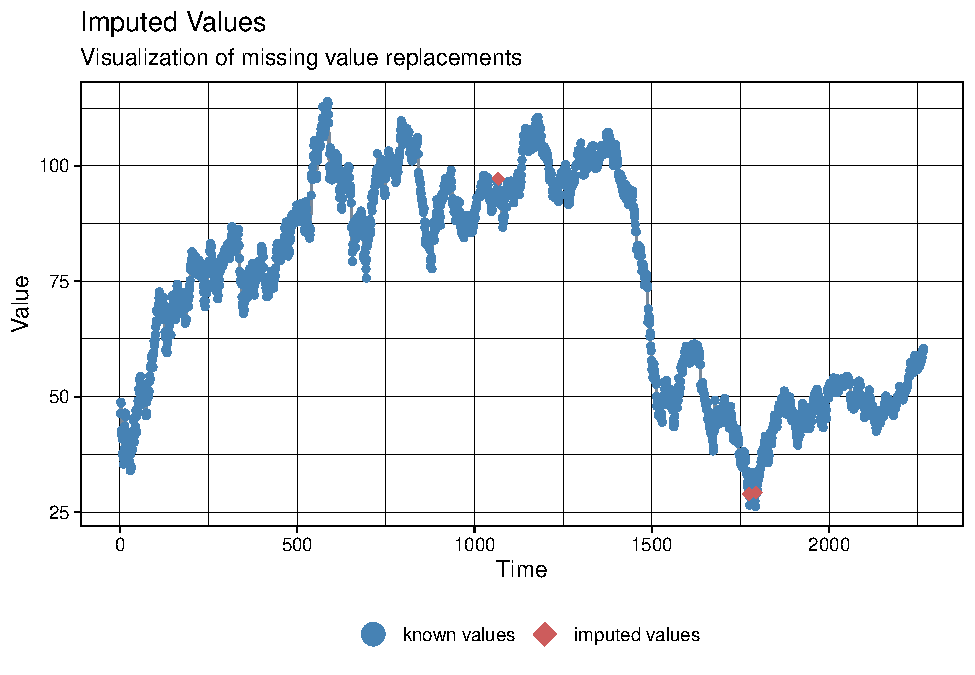
\includegraphics{_main_files/figure-latex/unnamed-chunk-7-1.pdf}

Untuk mengekstraksi peubah \emph{dummy} yang memodelkan efek hari setelah libur, buat sederet data yang berisi semua hari dari tahun 2009 sampai 2017, lalu merge:

\begin{Shaded}
\begin{Highlighting}[]
\FunctionTok{lazy\_dt}\NormalTok{(}\FunctionTok{seq}\NormalTok{(}\FunctionTok{as.Date}\NormalTok{(}\StringTok{"2009{-}01{-}01"}\NormalTok{), }\FunctionTok{as.Date}\NormalTok{(}\StringTok{"2017{-}12{-}31"}\NormalTok{), }\AttributeTok{by=}\StringTok{"days"}\NormalTok{)) }\SpecialCharTok{\%\textgreater{}\%}
  \FunctionTok{rename}\NormalTok{(}\AttributeTok{X=}\NormalTok{x) }\SpecialCharTok{\%\textgreater{}\%} \FunctionTok{left\_join}\NormalTok{(crude0917) }\SpecialCharTok{\%\textgreater{}\%} \FunctionTok{select}\NormalTok{(fixed) }\SpecialCharTok{\%\textgreater{}\%} 
  \FunctionTok{summarise}\NormalTok{(}\AttributeTok{ties =} \FunctionTok{sum}\NormalTok{(}\FunctionTok{is.na}\NormalTok{(.))) }\SpecialCharTok{\%\textgreater{}\%}\NormalTok{ knitr}\SpecialCharTok{::}\FunctionTok{kable}\NormalTok{(}\AttributeTok{col.names =} \StringTok{"Jumlah NA"}\NormalTok{)}
\end{Highlighting}
\end{Shaded}

\begin{tabular}{r}
\hline
Jumlah NA\\
\hline
1021\\
\hline
\end{tabular}

Terdapat 1021 data hilang. Buat deret hari akhir minggu dari tahun 2009 sampai 2017. Hari Sabtu pertama di dataset ini adalah Januari 3, 2009:

\begin{Shaded}
\begin{Highlighting}[]
\NormalTok{sats}\OtherTok{\textless{}{-}}\FunctionTok{seq}\NormalTok{(}\FunctionTok{as.Date}\NormalTok{(}\StringTok{"2009{-}01{-}03"}\NormalTok{), }\FunctionTok{as.Date}\NormalTok{(}\StringTok{"2017{-}12{-}31"}\NormalTok{), }\AttributeTok{by=}\StringTok{"weeks"}\NormalTok{)}
\NormalTok{suns}\OtherTok{\textless{}{-}}\FunctionTok{seq}\NormalTok{(}\FunctionTok{as.Date}\NormalTok{(}\StringTok{"2009{-}01{-}04"}\NormalTok{), }\FunctionTok{as.Date}\NormalTok{(}\StringTok{"2017{-}12{-}31"}\NormalTok{), }\AttributeTok{by=}\StringTok{"weeks"}\NormalTok{)}
\FunctionTok{length}\NormalTok{(}\FunctionTok{c}\NormalTok{(sats,suns))}
\end{Highlighting}
\end{Shaded}

\begin{verbatim}
## [1] 940
\end{verbatim}

Ada 940 hari yang merupakan akhir minggu dari 1024 hari libur. Untuk mendapat data hari libur nasional di bursa saham New York, gunakan fungsi \texttt{holidayNYSE} dari package \texttt{timeDate} (\protect\hyperlink{ref-R-timeDate}{Wuertz \emph{et al.} 2018}).

\begin{Shaded}
\begin{Highlighting}[]
\FunctionTok{library}\NormalTok{(timeDate)}
\FunctionTok{length}\NormalTok{(}\FunctionTok{as.Date}\NormalTok{(}\FunctionTok{holidayNYSE}\NormalTok{(}\AttributeTok{year=}\FunctionTok{seq}\NormalTok{(}\DecValTok{2009}\NormalTok{,}\DecValTok{2017}\NormalTok{,}\DecValTok{1}\NormalTok{))))}
\end{Highlighting}
\end{Shaded}

\begin{verbatim}
## [1] 80
\end{verbatim}

Terlihat bahwa 1020 dari data hilang dapat dijelaskan oleh libur nasional dan akhir minggu. Hanya 1 dari data hilang yang tidak dapat dijelaskan. Buat deret hari Senin dari tahun 2009 sampai 2017, dan hari setelah hari libur nasional. Gunakan package dplyr (\protect\hyperlink{ref-R-dplyr}{Wickham \emph{et al.} 2022}) untuk menghasilkan data.frame tersebut:

\begin{Shaded}
\begin{Highlighting}[]
\NormalTok{mons}\OtherTok{\textless{}{-}}\FunctionTok{lazy\_dt}\NormalTok{(suns}\SpecialCharTok{+}\DecValTok{1}\NormalTok{)}\SpecialCharTok{\%\textgreater{}\%}\FunctionTok{mutate}\NormalTok{(}\AttributeTok{dumMon=}\DecValTok{1}\NormalTok{)}
\NormalTok{posthol}\OtherTok{\textless{}{-}}\FunctionTok{lazy\_dt}\NormalTok{(}\FunctionTok{as.Date}\NormalTok{(}\FunctionTok{holidayNYSE}\NormalTok{(}\AttributeTok{year=}\FunctionTok{seq}\NormalTok{(}\DecValTok{2009}\NormalTok{,}\DecValTok{2017}\NormalTok{,}\DecValTok{1}\NormalTok{)))}\SpecialCharTok{+}\DecValTok{1}\NormalTok{) }\SpecialCharTok{\%\textgreater{}\%}
  \FunctionTok{mutate}\NormalTok{(}\AttributeTok{x=}\NormalTok{x}\SpecialCharTok{+}\DecValTok{1}\NormalTok{,}
        \AttributeTok{dumHol=}\DecValTok{1}\NormalTok{)}
\end{Highlighting}
\end{Shaded}

Lalu, merge data crude dengan data hari Senin dan hari setelah libur nasional.

\begin{Shaded}
\begin{Highlighting}[]
\NormalTok{crudeDummies}\OtherTok{\textless{}{-}}\NormalTok{ crude0917}\SpecialCharTok{\%\textgreater{}\%}
  \FunctionTok{left\_join}\NormalTok{(mons,}\AttributeTok{by=}\FunctionTok{c}\NormalTok{(}\StringTok{\textquotesingle{}X\textquotesingle{}}\OtherTok{=}\StringTok{\textquotesingle{}x\textquotesingle{}}\NormalTok{)) }\SpecialCharTok{\%\textgreater{}\%} \FunctionTok{left\_join}\NormalTok{(posthol,}\AttributeTok{by=}\FunctionTok{c}\NormalTok{(}\StringTok{\textquotesingle{}X\textquotesingle{}}\OtherTok{=}\StringTok{\textquotesingle{}x\textquotesingle{}}\NormalTok{)) }\SpecialCharTok{\%\textgreater{}\%}
  \FunctionTok{mutate}\NormalTok{(}\AttributeTok{dumMon=}\FunctionTok{ifelse}\NormalTok{(}\FunctionTok{is.na}\NormalTok{(dumMon),}\DecValTok{0}\NormalTok{,}\DecValTok{1}\NormalTok{),}
         \AttributeTok{dumHol=}\FunctionTok{ifelse}\NormalTok{(}\FunctionTok{is.na}\NormalTok{(dumHol),}\DecValTok{0}\NormalTok{,}\DecValTok{1}\NormalTok{))}
\end{Highlighting}
\end{Shaded}

Peubah \emph{dummy} untuk memodelkan efek pasar dibuka saat hari senin dan setelah libur telah dibuat. Peubah tersebut sebenarnya tidak terlalu berkorelasi dengan harga minyak, jadi mungkin saja efek-efek tersebut tidak ada:

\begin{Shaded}
\begin{Highlighting}[]
\NormalTok{crudeDummies }\SpecialCharTok{\%\textgreater{}\%} 
  \FunctionTok{summarize}\NormalTok{(}\AttributeTok{corHol=}\FunctionTok{cor}\NormalTok{(dumHol,fixed),}
            \AttributeTok{corMon=}\FunctionTok{cor}\NormalTok{(dumMon,fixed)) }\SpecialCharTok{\%\textgreater{}\%} 
\NormalTok{  knitr}\SpecialCharTok{::}\FunctionTok{kable}\NormalTok{(}\AttributeTok{col.names =} \FunctionTok{c}\NormalTok{(}\StringTok{"Senin"}\NormalTok{, }\StringTok{"Liburan"}\NormalTok{),}
               \AttributeTok{caption =} \StringTok{"Korelasi peubah dummy dengan harga minyak"}\NormalTok{)}
\end{Highlighting}
\end{Shaded}

\begin{table}

\caption{\label{tab:unnamed-chunk-13}Korelasi peubah dummy dengan harga minyak}
\centering
\begin{tabular}[t]{r|r}
\hline
Senin & Liburan\\
\hline
0.0038625 & -0.0022236\\
\hline
\end{tabular}
\end{table}

\hypertarget{pola-pola-data-dan-stasioneritas}{%
\section{Pola-pola data dan stasioneritas}\label{pola-pola-data-dan-stasioneritas}}

Plot dari data tersebut dibuat menggunakan \texttt{ggplot2} (\protect\hyperlink{ref-R-ggplot2}{Wickham \emph{et al.} 2021}):

\begin{Shaded}
\begin{Highlighting}[]
\FunctionTok{library}\NormalTok{(ggplot2)}

\NormalTok{data.table}\SpecialCharTok{::}\FunctionTok{as.data.table}\NormalTok{(crude0917) }\SpecialCharTok{\%\textgreater{}\%}
  \FunctionTok{ggplot}\NormalTok{(}\FunctionTok{aes}\NormalTok{(}\AttributeTok{x=}\NormalTok{X, }\AttributeTok{y=}\NormalTok{fixed)) }\SpecialCharTok{+}
      \FunctionTok{geom\_line}\NormalTok{()}\SpecialCharTok{+}
      \FunctionTok{ggtitle}\NormalTok{(}\StringTok{"Harga Minyak (CL.F. Close) {-} USD/Barrel"}\NormalTok{)}\SpecialCharTok{+}\FunctionTok{xlab}\NormalTok{(}\StringTok{"Waktu"}\NormalTok{)}\SpecialCharTok{+}\FunctionTok{ylab}\NormalTok{(}\StringTok{" "}\NormalTok{)}\SpecialCharTok{+}
      \FunctionTok{theme\_classic}\NormalTok{()}
\end{Highlighting}
\end{Shaded}

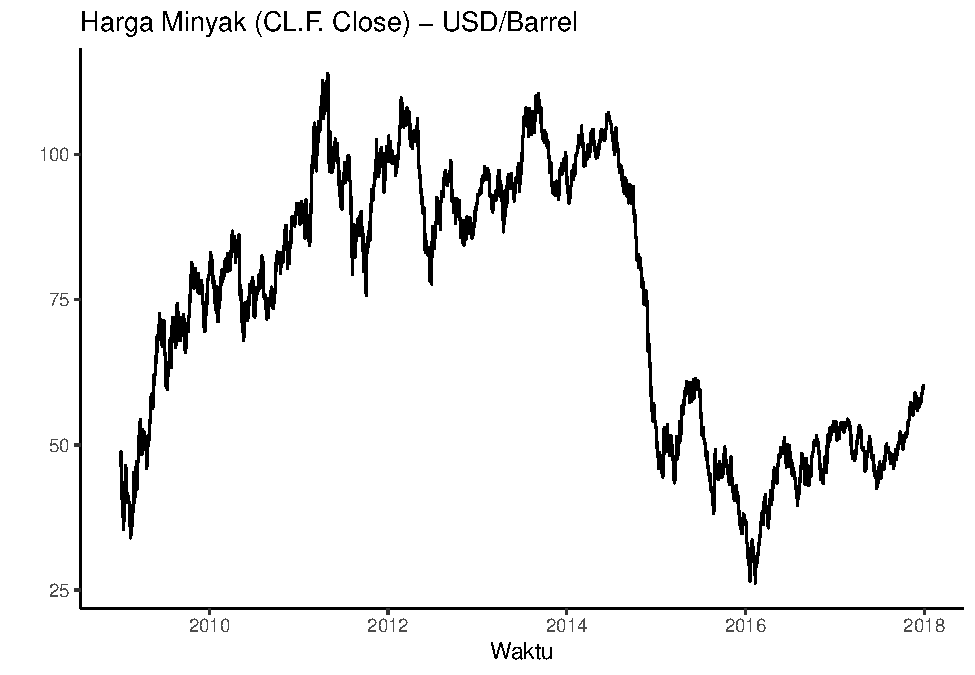
\includegraphics{_main_files/figure-latex/unnamed-chunk-14-1.pdf}

Terlihat bahwa data memiliki pola campuran. Secara kasar, terlihat tren naik pada tahun 2009-2011. Lalu, dari tahun 2011-2014 harga minyak siklik, tetapi rataannya tetap, kira-kira di atas 75 dolar. Harga minyak turun drastis dari tahun 2014-2016. Terakhir, harga minyak naik sedikit lalu stasioner lalu naik sedikit lagi di tahun 2016-2018. Pola-pola tersebut dapat dilihat setelah dilakukan segmentasi melalui \texttt{dplyr} (\protect\hyperlink{ref-R-dplyr}{Wickham \emph{et al.} 2022}). Segmentasi tersebut tidak dilakukan menggunakan metode formal, tetapi secara eksploratif saja:

\begin{Shaded}
\begin{Highlighting}[]
\FunctionTok{library}\NormalTok{(dplyr)}
\NormalTok{cbbPalette }\OtherTok{\textless{}{-}} \FunctionTok{c}\NormalTok{(}\StringTok{"\#000000"}\NormalTok{, }\StringTok{"\#E69F00"}\NormalTok{, }\StringTok{"\#56B4E9"}\NormalTok{, }\StringTok{"\#009E73"}\NormalTok{, }
                \StringTok{"\#F0E442"}\NormalTok{, }\StringTok{"\#0072B2"}\NormalTok{, }\StringTok{"\#D55E00"}\NormalTok{, }\StringTok{"\#CC79A7"}\NormalTok{)}
\CommentTok{\#palet yang inklusif pada buta warna}

\NormalTok{crude0917 }\SpecialCharTok{\%\textgreater{}\%}
  \FunctionTok{mutate}\NormalTok{(}\AttributeTok{Segmen=}
           \FunctionTok{ifelse}\NormalTok{(X}\SpecialCharTok{\textless{}=}\FunctionTok{as.Date}\NormalTok{(}\StringTok{\textquotesingle{}2010{-}12{-}31\textquotesingle{}}\NormalTok{),}\StringTok{"1"}\NormalTok{,}
           \FunctionTok{ifelse}\NormalTok{(X}\SpecialCharTok{\textless{}=}\FunctionTok{as.Date}\NormalTok{(}\StringTok{\textquotesingle{}2014{-}06{-}01\textquotesingle{}}\NormalTok{),}\StringTok{"2"}\NormalTok{,}
           \FunctionTok{ifelse}\NormalTok{(X}\SpecialCharTok{\textless{}=}\FunctionTok{as.Date}\NormalTok{(}\StringTok{\textquotesingle{}2016{-}01{-}01\textquotesingle{}}\NormalTok{),}\StringTok{"3"}\NormalTok{,}\StringTok{"4"}\NormalTok{)))}\CommentTok{\#buat segmentasi }
\NormalTok{  )}\SpecialCharTok{\%\textgreater{}\%}\NormalTok{ data.table}\SpecialCharTok{::}\FunctionTok{as.data.table}\NormalTok{()}\SpecialCharTok{\%\textgreater{}\%}
  \FunctionTok{ggplot}\NormalTok{(}\FunctionTok{aes}\NormalTok{(}\AttributeTok{x=}\NormalTok{X,}\AttributeTok{y=}\NormalTok{fixed))}\SpecialCharTok{+}
    \FunctionTok{geom\_line}\NormalTok{(}\FunctionTok{aes}\NormalTok{(}\AttributeTok{color=}\NormalTok{Segmen))}\SpecialCharTok{+}\FunctionTok{scale\_color\_manual}\NormalTok{(}\AttributeTok{values=}\NormalTok{cbbPalette)}\SpecialCharTok{+}
    \FunctionTok{ggtitle}\NormalTok{(}\StringTok{"Segmentasi Harga Minyak (CL.F Close) {-} USD/Barrel"}\NormalTok{)}\SpecialCharTok{+}
    \FunctionTok{xlab}\NormalTok{(}\StringTok{"Waktu"}\NormalTok{)}\SpecialCharTok{+}\FunctionTok{ylab}\NormalTok{(}\StringTok{" "}\NormalTok{)}\SpecialCharTok{+}\FunctionTok{theme\_classic}\NormalTok{()}
\end{Highlighting}
\end{Shaded}

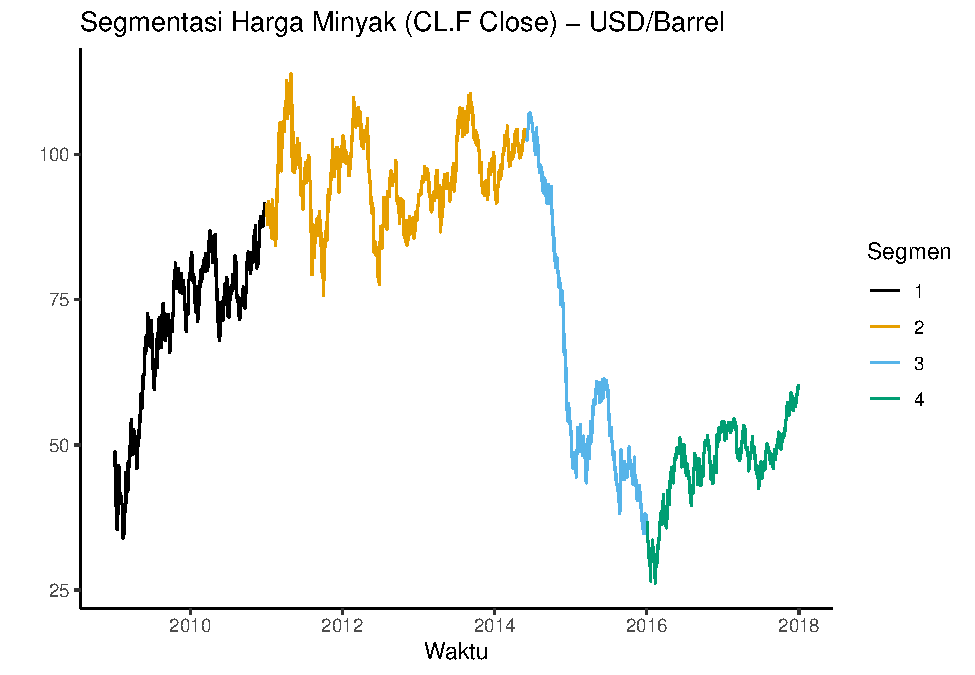
\includegraphics{_main_files/figure-latex/unnamed-chunk-15-1.pdf}

Namun, sebenarnya segmentasi ini belum terlalu detail. Misal, sebenarnya harga minyak naik dari tahun 2009 ke 2010, lalu mengalami pola siklik dari tahun 2010 ke 2011. Kekasasaran segmentasi ini dapat dilihat dari boxplot. Masih banyak titik-titik yang di luar garis (whisker), yang menandandakan ada banyak amatan ekstrim:

\begin{Shaded}
\begin{Highlighting}[]
\NormalTok{crude0917 }\SpecialCharTok{\%\textgreater{}\%}
  \FunctionTok{mutate}\NormalTok{(}\AttributeTok{Segmen=}
           \FunctionTok{ifelse}\NormalTok{(X}\SpecialCharTok{\textless{}=}\FunctionTok{as.Date}\NormalTok{(}\StringTok{\textquotesingle{}2010{-}12{-}31\textquotesingle{}}\NormalTok{),}\StringTok{"1"}\NormalTok{,}
           \FunctionTok{ifelse}\NormalTok{(X}\SpecialCharTok{\textless{}=}\FunctionTok{as.Date}\NormalTok{(}\StringTok{\textquotesingle{}2014{-}06{-}01\textquotesingle{}}\NormalTok{),}\StringTok{"2"}\NormalTok{,}
           \FunctionTok{ifelse}\NormalTok{(X}\SpecialCharTok{\textless{}=}\FunctionTok{as.Date}\NormalTok{(}\StringTok{\textquotesingle{}2016{-}01{-}01\textquotesingle{}}\NormalTok{),}\StringTok{"3"}\NormalTok{,}\StringTok{"4"}\NormalTok{)))}\CommentTok{\#buat segmentasi }
\NormalTok{  )}\SpecialCharTok{\%\textgreater{}\%}\NormalTok{ data.table}\SpecialCharTok{::}\FunctionTok{as.data.table}\NormalTok{()}\SpecialCharTok{\%\textgreater{}\%}
  \FunctionTok{ggplot}\NormalTok{(}\FunctionTok{aes}\NormalTok{(}\AttributeTok{x=}\NormalTok{X,}\AttributeTok{y=}\NormalTok{fixed))}\SpecialCharTok{+}
    \FunctionTok{geom\_boxplot}\NormalTok{(}\FunctionTok{aes}\NormalTok{(}\AttributeTok{fill=}\NormalTok{Segmen))}\SpecialCharTok{+}\FunctionTok{scale\_fill\_manual}\NormalTok{(}\AttributeTok{values=}\NormalTok{cbbPalette)}\SpecialCharTok{+}
    \FunctionTok{xlab}\NormalTok{(}\StringTok{"Waktu"}\NormalTok{)}\SpecialCharTok{+}\FunctionTok{ylab}\NormalTok{(}\StringTok{" "}\NormalTok{)}\SpecialCharTok{+}\FunctionTok{theme\_classic}\NormalTok{()}
\end{Highlighting}
\end{Shaded}

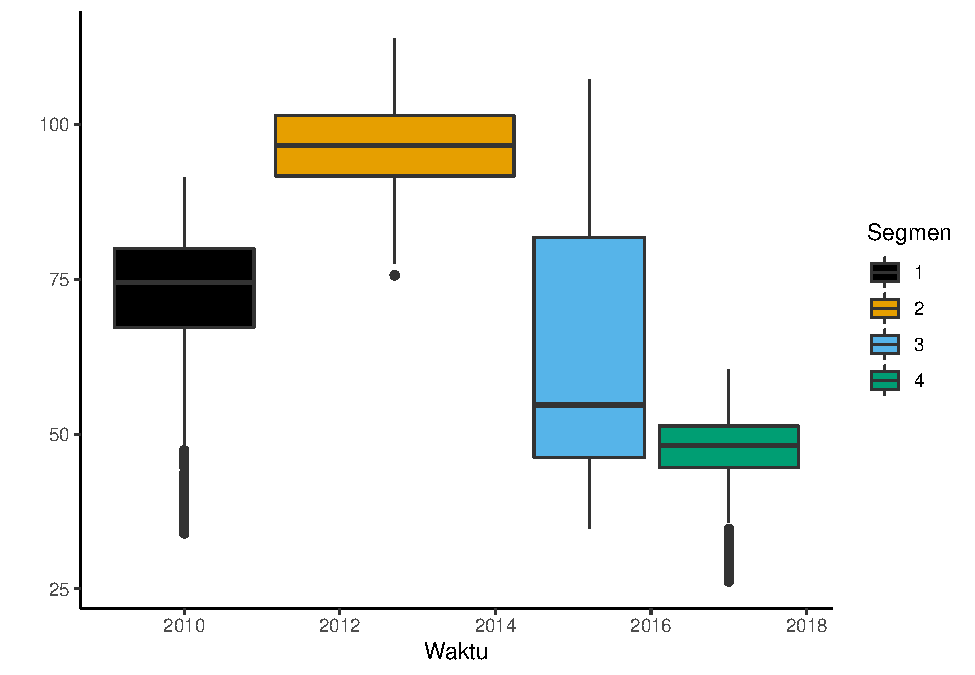
\includegraphics{_main_files/figure-latex/unnamed-chunk-16-1.pdf}

Selain detail pertama yang disebutkan di atas, terlihat bahwa di penurunan harga minyak tahun 2014-2016, sempat ada kenaikan sedikit lalu turun lagi. Dengan menambahkan segmen-segmen tersebut, segmentasi yang detail adalah:

\begin{Shaded}
\begin{Highlighting}[]
\NormalTok{crude0917 }\SpecialCharTok{\%\textgreater{}\%}
  \FunctionTok{mutate}\NormalTok{(}\AttributeTok{Segmen=}
          \FunctionTok{ifelse}\NormalTok{(X}\SpecialCharTok{\textless{}=}\FunctionTok{as.Date}\NormalTok{(}\StringTok{\textquotesingle{}2009{-}10{-}01\textquotesingle{}}\NormalTok{),}\StringTok{"1"}\NormalTok{,}
          \FunctionTok{ifelse}\NormalTok{(X}\SpecialCharTok{\textless{}=}\FunctionTok{as.Date}\NormalTok{(}\StringTok{\textquotesingle{}2010{-}10{-}31\textquotesingle{}}\NormalTok{),}\StringTok{"2"}\NormalTok{,}
          \FunctionTok{ifelse}\NormalTok{(X}\SpecialCharTok{\textless{}=}\FunctionTok{as.Date}\NormalTok{(}\StringTok{\textquotesingle{}2014{-}06{-}30\textquotesingle{}}\NormalTok{),}\StringTok{"3"}\NormalTok{,}
          \FunctionTok{ifelse}\NormalTok{(X}\SpecialCharTok{\textless{}=}\FunctionTok{as.Date}\NormalTok{(}\StringTok{\textquotesingle{}2015{-}02{-}01\textquotesingle{}}\NormalTok{),}\StringTok{"4"}\NormalTok{,}
          \FunctionTok{ifelse}\NormalTok{(X}\SpecialCharTok{\textless{}=}\FunctionTok{as.Date}\NormalTok{(}\StringTok{\textquotesingle{}2016{-}05{-}01\textquotesingle{}}\NormalTok{),}\StringTok{"6"}\NormalTok{,}\StringTok{"7"}\NormalTok{)}
\NormalTok{          ))))}\CommentTok{\#buat segmentasi }
\NormalTok{  )}\SpecialCharTok{\%\textgreater{}\%}\NormalTok{ data.table}\SpecialCharTok{::}\FunctionTok{as.data.table}\NormalTok{() }\SpecialCharTok{\%\textgreater{}\%}
  \FunctionTok{ggplot}\NormalTok{(}\FunctionTok{aes}\NormalTok{(}\AttributeTok{x=}\NormalTok{X,}\AttributeTok{y=}\NormalTok{fixed))}\SpecialCharTok{+}
  \FunctionTok{geom\_line}\NormalTok{(}\FunctionTok{aes}\NormalTok{(}\AttributeTok{color=}\NormalTok{Segmen))}\SpecialCharTok{+}\FunctionTok{scale\_color\_manual}\NormalTok{(}\AttributeTok{values=}\NormalTok{cbbPalette)}\SpecialCharTok{+}
  \FunctionTok{ggtitle}\NormalTok{(}\StringTok{"Segmentasi Detail Harga Minyak (CL.F Close) {-} USD/Barrel"}\NormalTok{)}\SpecialCharTok{+}
  \FunctionTok{xlab}\NormalTok{(}\StringTok{"Waktu"}\NormalTok{)}\SpecialCharTok{+}\FunctionTok{ylab}\NormalTok{(}\StringTok{" "}\NormalTok{)}\SpecialCharTok{+}
  \FunctionTok{theme\_classic}\NormalTok{()}
\end{Highlighting}
\end{Shaded}

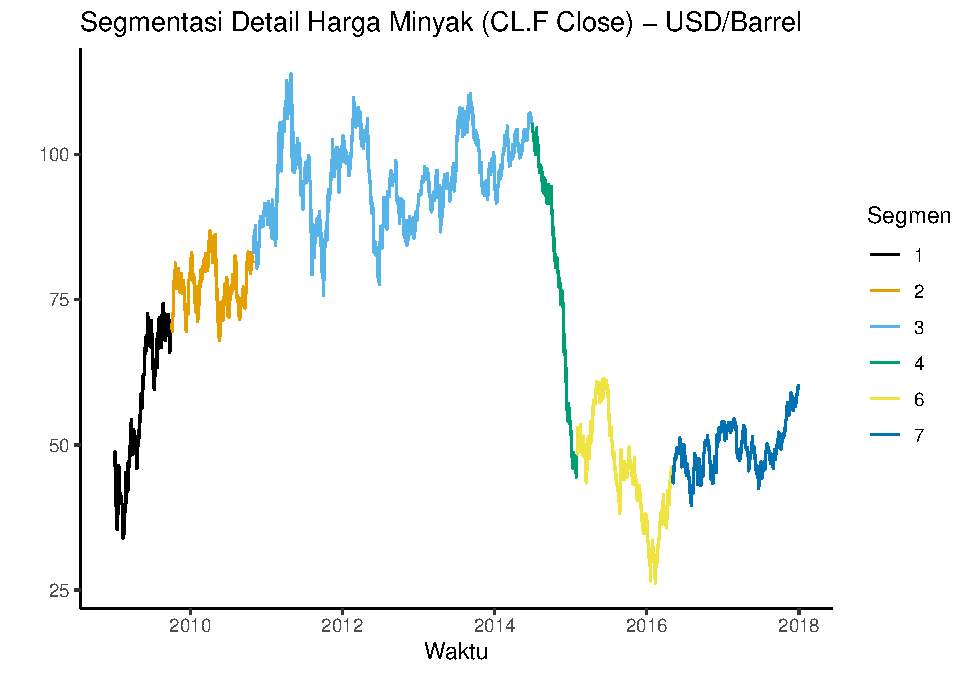
\includegraphics{_main_files/figure-latex/unnamed-chunk-17-1.pdf}

Dapat dilihat dari boxplot per kelompok segmentasi tersebut bahwa sama sekali tidak ada amatan ekstrim yang menandakan bahwa pengelompokan sudah baik.

\begin{Shaded}
\begin{Highlighting}[]
\NormalTok{crude0917 }\SpecialCharTok{\%\textgreater{}\%}
  \FunctionTok{mutate}\NormalTok{(}\AttributeTok{Segmen=}
          \FunctionTok{ifelse}\NormalTok{(X}\SpecialCharTok{\textless{}=}\FunctionTok{as.Date}\NormalTok{(}\StringTok{\textquotesingle{}2009{-}10{-}01\textquotesingle{}}\NormalTok{),}\StringTok{"1"}\NormalTok{,}
          \FunctionTok{ifelse}\NormalTok{(X}\SpecialCharTok{\textless{}=}\FunctionTok{as.Date}\NormalTok{(}\StringTok{\textquotesingle{}2010{-}10{-}31\textquotesingle{}}\NormalTok{),}\StringTok{"2"}\NormalTok{,}
          \FunctionTok{ifelse}\NormalTok{(X}\SpecialCharTok{\textless{}=}\FunctionTok{as.Date}\NormalTok{(}\StringTok{\textquotesingle{}2014{-}06{-}30\textquotesingle{}}\NormalTok{),}\StringTok{"3"}\NormalTok{,}
          \FunctionTok{ifelse}\NormalTok{(X}\SpecialCharTok{\textless{}=}\FunctionTok{as.Date}\NormalTok{(}\StringTok{\textquotesingle{}2015{-}02{-}01\textquotesingle{}}\NormalTok{),}\StringTok{"4"}\NormalTok{,}
          \FunctionTok{ifelse}\NormalTok{(X}\SpecialCharTok{\textless{}=}\FunctionTok{as.Date}\NormalTok{(}\StringTok{\textquotesingle{}2016{-}05{-}01\textquotesingle{}}\NormalTok{),}\StringTok{"6"}\NormalTok{,}\StringTok{"7"}\NormalTok{)}
\NormalTok{          ))))}\CommentTok{\#buat segmentasi }
\NormalTok{  )}\SpecialCharTok{\%\textgreater{}\%}\NormalTok{ data.table}\SpecialCharTok{::}\FunctionTok{as.data.table}\NormalTok{() }\SpecialCharTok{\%\textgreater{}\%}
  \FunctionTok{ggplot}\NormalTok{(}\FunctionTok{aes}\NormalTok{(}\AttributeTok{x=}\NormalTok{X,}\AttributeTok{y=}\NormalTok{fixed))}\SpecialCharTok{+}
  \FunctionTok{geom\_boxplot}\NormalTok{(}\FunctionTok{aes}\NormalTok{(}\AttributeTok{fill=}\NormalTok{Segmen))}\SpecialCharTok{+}\FunctionTok{scale\_fill\_manual}\NormalTok{(}\AttributeTok{values=}\NormalTok{cbbPalette)}\SpecialCharTok{+}
  \FunctionTok{ggtitle}\NormalTok{(}\StringTok{"Boxplot per Segmen Harga Minyak (CL.F Close)"}\NormalTok{)}\SpecialCharTok{+}\FunctionTok{xlab}\NormalTok{(}\StringTok{"Waktu"}\NormalTok{)}\SpecialCharTok{+}\FunctionTok{ylab}\NormalTok{(}\StringTok{" "}\NormalTok{)}\SpecialCharTok{+}
  \FunctionTok{theme\_classic}\NormalTok{()}
\end{Highlighting}
\end{Shaded}

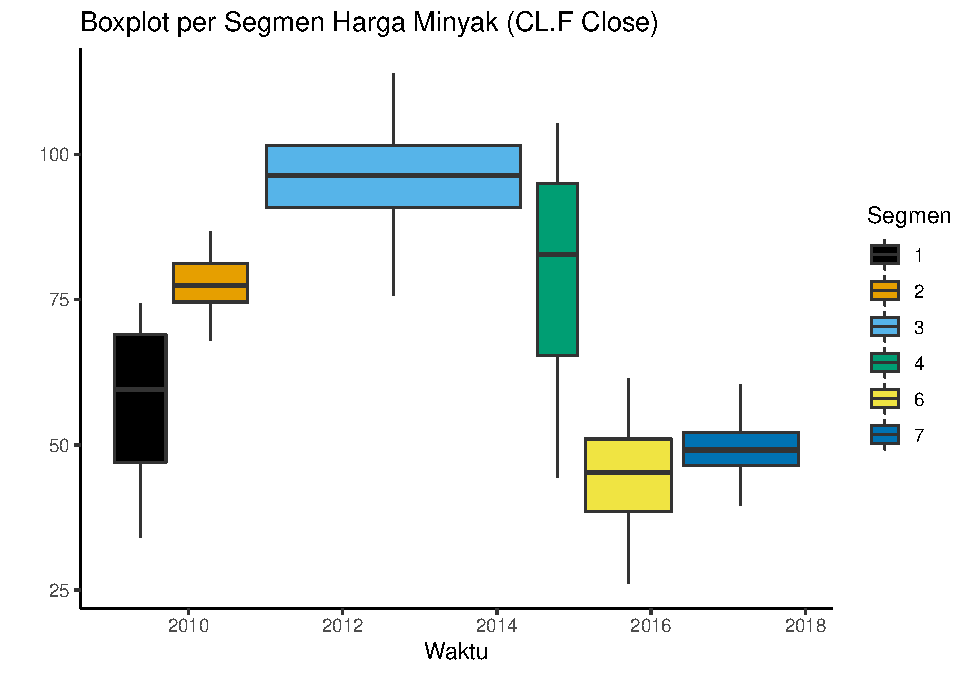
\includegraphics{_main_files/figure-latex/unnamed-chunk-18-1.pdf}

\hypertarget{latar-belakang}{%
\section{Latar Belakang}\label{latar-belakang}}

Variasi dari segmen tersebut dapat dijelaskan dengan beberapa faktor perubahan harga minyak, yaitu perubahan penawaran dan permintaan minyak mentah karena konflik yang melibatkan negara-negara penghasil minyak dan krisis ekonomi yang melanda negara-negara besar.

\hypertarget{harga-minyak-mentah-tahun-2009}{%
\subsection{Harga Minyak Mentah Tahun 2009}\label{harga-minyak-mentah-tahun-2009}}

Harga minyak pada awal 2009 sangat rendah karena efek krisis finansial yang melanda Amerika Serikat dan Eropa pada tahun 2008. Krisis finansial tersebut terjadi karena krisis pinjaman kredit yang terjadi di Amerika Serikat. Akibatnya, berbagai bank di Amerika Serikat bangkrut dan ekonomi dunia melemah. Setelah itu, permintaan minyak mentah juga melemah (karena minyak merupakan input besar di ekonomi dunia) dan harga minyak mentah turun dari titik tertinggi, yaitu 133.88 USD pada Juni 2008 ke 39.09 USD per barrel pada Februari 2009 (\protect\hyperlink{ref-tlioil}{Li 2021}).

Pemerintah Amerika Serikat memberikan respons terhadap krisis tersebut dengan memberikan stimulus kepada pasar finansial seperti bank yang mengalami krisis keuangan. Akhirnya, ekonomi pada pertengahan 2009 mulai pulih dan permintaan minyak mentah meningkat kembali menjadi sekitar 70 USD per barrel pada Juni 2009 (\protect\hyperlink{ref-guardoil}{Wearden 2009}). Terlihat bahwa dari periode Januari 2009 sampai Desember 2010, harga kontrak berjangka minyak naik:

\begin{Shaded}
\begin{Highlighting}[]
\NormalTok{highlightPalette}\OtherTok{\textless{}{-}}\FunctionTok{c}\NormalTok{( }\StringTok{"\#56B4E9"}\NormalTok{,}\StringTok{"\#D55E00"}\NormalTok{,}\StringTok{"\#D3D3D3"}\NormalTok{)}

\NormalTok{crude0917 }\SpecialCharTok{\%\textgreater{}\%}
  \FunctionTok{mutate}\NormalTok{(}\AttributeTok{Keterangan=}
          \FunctionTok{ifelse}\NormalTok{(X}\SpecialCharTok{\textless{}=}\FunctionTok{as.Date}\NormalTok{(}\StringTok{\textquotesingle{}2009{-}06{-}01\textquotesingle{}}\NormalTok{),}
                 \StringTok{"Jan 2009 {-} Jun 2009 (Pemulihan Harga)"}\NormalTok{,}
          \FunctionTok{ifelse}\NormalTok{(X}\SpecialCharTok{\textless{}=}\FunctionTok{as.Date}\NormalTok{(}\StringTok{\textquotesingle{}2010{-}12{-}17\textquotesingle{}}\NormalTok{),}
                 \StringTok{"Harga Stabil Sebelum Arab Spring"}\NormalTok{,}
                  \StringTok{"Lainnya"}\NormalTok{))}\CommentTok{\#buat segmentasi }
\NormalTok{  )}\SpecialCharTok{\%\textgreater{}\%}\NormalTok{ data.table}\SpecialCharTok{::}\FunctionTok{as.data.table}\NormalTok{() }\SpecialCharTok{\%\textgreater{}\%}
  \FunctionTok{ggplot}\NormalTok{(}\FunctionTok{aes}\NormalTok{(}\AttributeTok{x=}\NormalTok{X,}\AttributeTok{y=}\NormalTok{fixed))}\SpecialCharTok{+}
  \FunctionTok{geom\_line}\NormalTok{(}\FunctionTok{aes}\NormalTok{(}\AttributeTok{color=}\NormalTok{Keterangan))}\SpecialCharTok{+}\FunctionTok{scale\_color\_manual}\NormalTok{(}\AttributeTok{values=}\NormalTok{highlightPalette)}\SpecialCharTok{+}
  \FunctionTok{ggtitle}\NormalTok{(}\StringTok{"Harga Minyak Setelah Krisis 2008"}\NormalTok{)}\SpecialCharTok{+}
  \FunctionTok{xlab}\NormalTok{(}\StringTok{"Waktu"}\NormalTok{)}\SpecialCharTok{+}\FunctionTok{ylab}\NormalTok{(}\StringTok{" "}\NormalTok{)}\SpecialCharTok{+}
  \FunctionTok{theme\_classic}\NormalTok{()}
\end{Highlighting}
\end{Shaded}

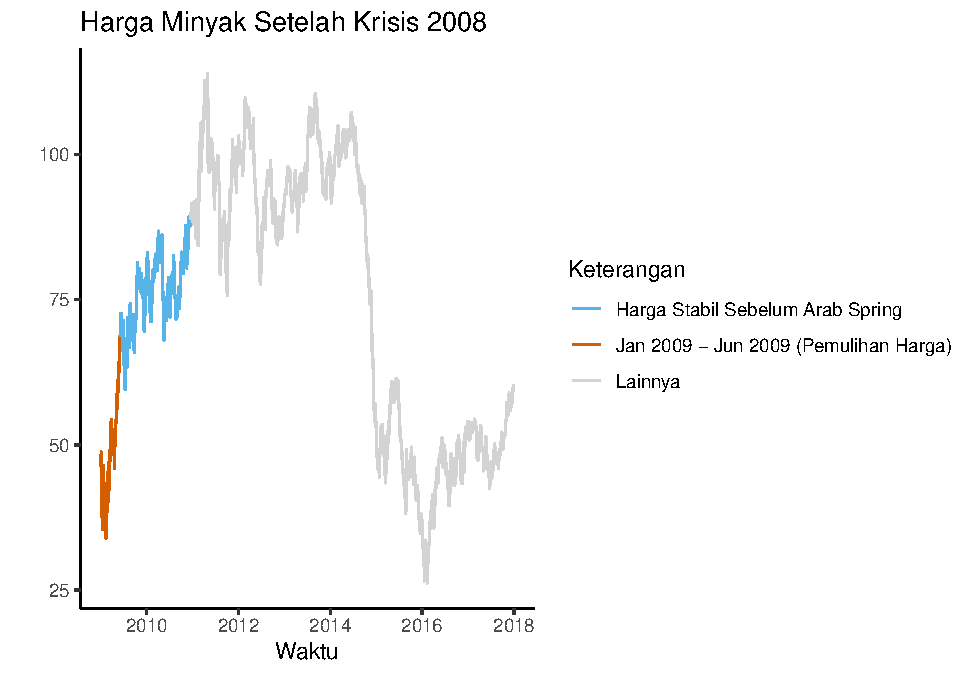
\includegraphics{_main_files/figure-latex/unnamed-chunk-19-1.pdf}

\hypertarget{arab-spring}{%
\subsection{Arab Spring}\label{arab-spring}}

Peristiwa ``Arab Spring'' merupakan peristiwa politik yang terjadi di negara-negara Arab, seperti Mesir, Libya, Tunisia, dan lain-lain. Peristiwa tersebut dimulai sejak awal tahun 2011 yang menjadi titik awal perubahan sistem tatanan politik yang demokratis di negara-negara tersebut. Arab Spring memberikan implikasi penting terhadap pasar minyak internasional (\protect\hyperlink{ref-khan_economic_2014}{Khan 2014}). Konflik yang terjadi negara-negara Arab tersebut (yang merupakan pengekspor minyak terbesar) yang mengganggu proses produksi dan ekspor minyak dan gas bahkan turun sampai nol. Turunnya produksi tersebut yang biasanya menyumbang 5\% dari produksi global mengakibatkan harga naik di seluruh dunia. Oleh karena itu, harga minyak siklik di atas 75 dolar per barrel pada waktu tersebut.

\begin{Shaded}
\begin{Highlighting}[]
\NormalTok{highlightPalette}\OtherTok{\textless{}{-}}\FunctionTok{c}\NormalTok{(}\StringTok{"\#56B4E9"}\NormalTok{,}\StringTok{"\#D3D3D3"}\NormalTok{,}\StringTok{"\#D3D3D3"}\NormalTok{)}

\NormalTok{crude0917 }\SpecialCharTok{\%\textgreater{}\%}
  \FunctionTok{mutate}\NormalTok{(}\AttributeTok{Keterangan=}
           \FunctionTok{ifelse}\NormalTok{(X}\SpecialCharTok{\textless{}=}\FunctionTok{as.Date}\NormalTok{(}\StringTok{\textquotesingle{}2010{-}12{-}17\textquotesingle{}}\NormalTok{), }\StringTok{"Sebelum Arab Spring"}\NormalTok{,}
           \FunctionTok{ifelse}\NormalTok{(X}\SpecialCharTok{\textless{}=}\FunctionTok{as.Date}\NormalTok{(}\StringTok{\textquotesingle{}2012{-}12{-}31\textquotesingle{}}\NormalTok{),}\StringTok{"Arab Spring"}\NormalTok{,}
            \StringTok{"Lainnya"}\NormalTok{))}\CommentTok{\#buat segmentasi }
\NormalTok{  )}\SpecialCharTok{\%\textgreater{}\%}\NormalTok{ data.table}\SpecialCharTok{::}\FunctionTok{as.data.table}\NormalTok{() }\SpecialCharTok{\%\textgreater{}\%}
  \FunctionTok{ggplot}\NormalTok{(}\FunctionTok{aes}\NormalTok{(}\AttributeTok{x=}\NormalTok{X,}\AttributeTok{y=}\NormalTok{fixed))}\SpecialCharTok{+}
  \FunctionTok{geom\_line}\NormalTok{(}\FunctionTok{aes}\NormalTok{(}\AttributeTok{color=}\NormalTok{Keterangan))}\SpecialCharTok{+}\FunctionTok{scale\_color\_manual}\NormalTok{(}\AttributeTok{values=}\NormalTok{highlightPalette)}\SpecialCharTok{+}
  \FunctionTok{ggtitle}\NormalTok{(}\StringTok{"Harga Minyak saat Arab Spring"}\NormalTok{)}\SpecialCharTok{+}
  \FunctionTok{xlab}\NormalTok{(}\StringTok{"Waktu"}\NormalTok{)}\SpecialCharTok{+}\FunctionTok{ylab}\NormalTok{(}\StringTok{" "}\NormalTok{)}\SpecialCharTok{+}
  \FunctionTok{theme\_classic}\NormalTok{()}
\end{Highlighting}
\end{Shaded}

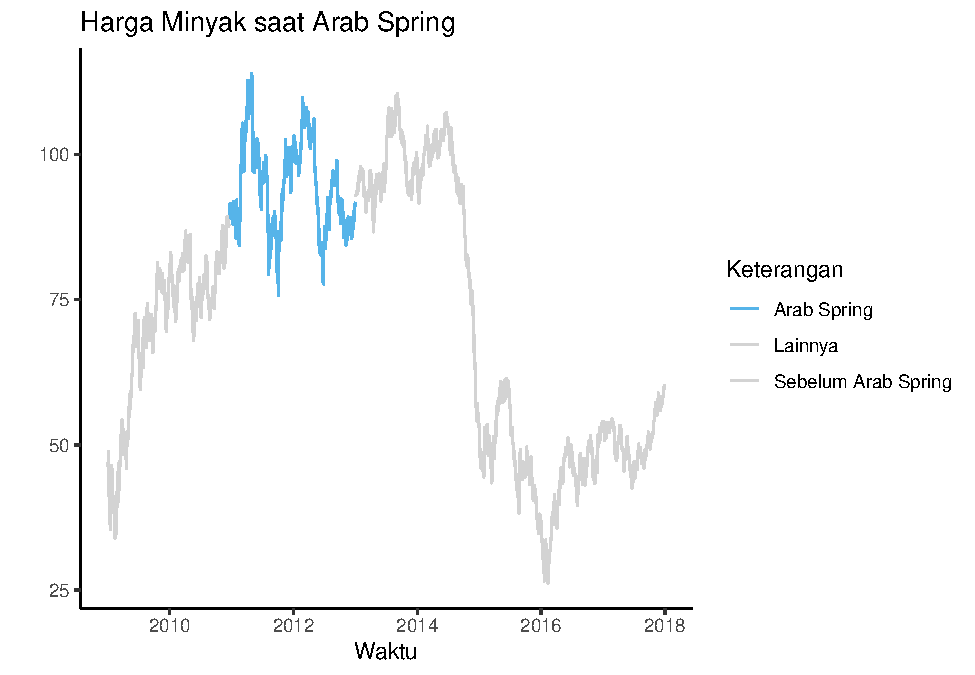
\includegraphics{_main_files/figure-latex/unnamed-chunk-20-1.pdf}

Selain ketidakstabilan yang disebabkan Arab Spring, pertumbuhan ekonomi di Tiongkok meningkatkan permintaan minyak sehingga terdapat tekanan dalam permintaan dan penawaran untuk meningatkan harga minyak (\protect\hyperlink{ref-voxoil}{Plumer 2014}).

\hypertarget{shale-revolution}{%
\subsection{Shale Revolution}\label{shale-revolution}}

``Shale Revolution'' mengacu pada kombinasi rekahan hidrolik dan pengeboran horizontal yang memungkinkan Amerika Serikat untuk secara signifikan meningkatkan produksi minyak dan gas alamnya, terutama dari formasi minyak ketat, yang sekarang mencapai 36\% dari total produksi minyak mentah AS. Kapasitas produksi baru ini telah mengurangi ketergantungan Amerika Serikat pada impor minyak dari luar negeri dan terus memberikan dorongan ekonomi yang penting saat negara itu pulih dari resesi 2008. Minyak dan gas merupakan 1,6\% dari PDB Amerika Serikat pada tahun 2011 dan terus berkembang. Perkembangan formasi serpih telah berkorelasi dengan peningkatan lapangan kerja, dengan industri minyak dan gas menambahkan 169.000 pekerjaan antara 2010 dan 2012.

\begin{Shaded}
\begin{Highlighting}[]
\NormalTok{highlightPalette}\OtherTok{\textless{}{-}}\FunctionTok{c}\NormalTok{(}\StringTok{"\#D3D3D3"}\NormalTok{,}\StringTok{"\#D3D3D3"}\NormalTok{,}\StringTok{"\#56B4E9"}\NormalTok{)}

\NormalTok{crude0917 }\SpecialCharTok{\%\textgreater{}\%}
  \FunctionTok{mutate}\NormalTok{(}\AttributeTok{Keterangan=}
           \FunctionTok{ifelse}\NormalTok{(X}\SpecialCharTok{\textless{}=}\FunctionTok{as.Date}\NormalTok{(}\StringTok{\textquotesingle{}2014{-}01{-}01\textquotesingle{}}\NormalTok{), }\StringTok{"Sebelum Shale Revolution"}\NormalTok{,}
           \FunctionTok{ifelse}\NormalTok{(X}\SpecialCharTok{\textless{}=}\FunctionTok{as.Date}\NormalTok{(}\StringTok{\textquotesingle{}2016{-}01{-}01\textquotesingle{}}\NormalTok{),}\StringTok{"Shale Revolution"}\NormalTok{,}
                                          \StringTok{"Setelah Shale Revolution"}\NormalTok{))}
         \CommentTok{\#buat segmentasi }
\NormalTok{  )}\SpecialCharTok{\%\textgreater{}\%}\NormalTok{data.table}\SpecialCharTok{::}\FunctionTok{as.data.table}\NormalTok{() }\SpecialCharTok{\%\textgreater{}\%}
  \FunctionTok{ggplot}\NormalTok{(}\FunctionTok{aes}\NormalTok{(}\AttributeTok{x=}\NormalTok{X,}\AttributeTok{y=}\NormalTok{fixed))}\SpecialCharTok{+}
  \FunctionTok{geom\_line}\NormalTok{(}\FunctionTok{aes}\NormalTok{(}\AttributeTok{color=}\NormalTok{Keterangan))}\SpecialCharTok{+}\FunctionTok{scale\_color\_manual}\NormalTok{(}\AttributeTok{values=}\NormalTok{highlightPalette)}\SpecialCharTok{+}
  \FunctionTok{ggtitle}\NormalTok{(}\StringTok{"Penurunan Harga Minyak 2014{-}2016"}\NormalTok{)}\SpecialCharTok{+}
  \FunctionTok{xlab}\NormalTok{(}\StringTok{"Waktu"}\NormalTok{)}\SpecialCharTok{+}\FunctionTok{ylab}\NormalTok{(}\StringTok{" "}\NormalTok{)}\SpecialCharTok{+}
  \FunctionTok{theme\_classic}\NormalTok{()}
\end{Highlighting}
\end{Shaded}

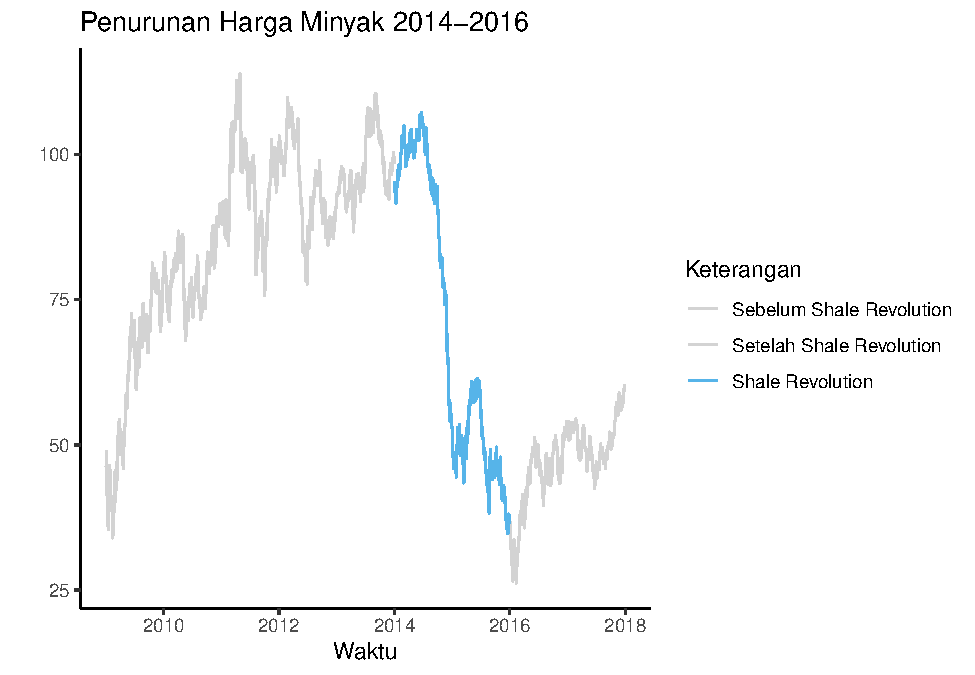
\includegraphics{_main_files/figure-latex/unnamed-chunk-21-1.pdf}

Perkembangan industri minyak dan gas tersebut meningkatkan produksi minyak dunia. Selain itu, negara-negara produsen minyak di OPEC mempertahankan atau meningkatkan produksi minyak mentah yang. Permintaan minyak di beberapa negara seperti Tiongkok dan di Uni Eropa juga menurun, sehingga faktor-faktor tersebut menurunkan harga minyak pada periode 2014-2016. Harga minyak mentah dunia mengalami penurunan pada akhir tahun 2014 dari US\$100 per barel hingga US\$40 per barel pada tahun 2016 dan mulai naik pada tahun 2017 (\protect\hyperlink{ref-mead_2014_2015}{Mead dan Stiger 2015}).

\hypertarget{titik-titik-perubahan-struktural}{%
\section{Titik-titik perubahan struktural}\label{titik-titik-perubahan-struktural}}

Secara lebih formal, dapat dicari titik-titik perubahan struktural di deret waktu tersebut menggunakan fungsi \texttt{breakpoints} dari package \texttt{strucchange} (\protect\hyperlink{ref-R-strucchange}{Zeileis \emph{et al.} 2019}). Algoritma yang dipakai cukup sederhana: dihitung BIC dan Jumlah Kuadrat Sisaan di tiap kemungkinan titik perubahan struktural. ika kita menggunakan model rata-rata yang sederhana seperti \texttt{lm(y\textasciitilde{}1)}, terlihat bahwa dibutuhkan dua break point untuk data tersebut:

\begin{Shaded}
\begin{Highlighting}[]
\FunctionTok{library}\NormalTok{(strucchangeRcpp)}

\NormalTok{breakOil}\OtherTok{\textless{}{-}}\FunctionTok{breakpoints}\NormalTok{(}\FunctionTok{pull}\NormalTok{(crude0917,fixed)}\SpecialCharTok{\textasciitilde{}}\DecValTok{1}\NormalTok{)}
\FunctionTok{plot}\NormalTok{(breakOil)}
\end{Highlighting}
\end{Shaded}

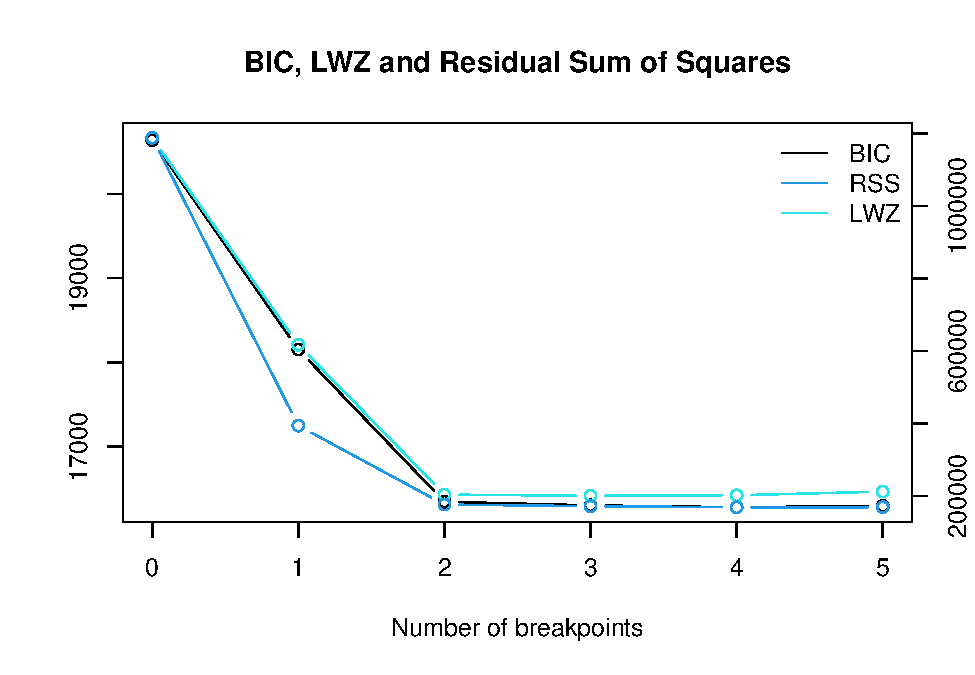
\includegraphics{_main_files/figure-latex/unnamed-chunk-22-1.pdf}

RSS dan BIC turun drastis setelah menambah dua break point. Break point tersebut dapat diperlihatkan sebagai berikut:

\begin{Shaded}
\begin{Highlighting}[]
\FunctionTok{breakpoints}\NormalTok{(}\FunctionTok{pull}\NormalTok{(crude0917,fixed)}\SpecialCharTok{\textasciitilde{}}\DecValTok{1}\NormalTok{,}\AttributeTok{breaks=}\DecValTok{2}\NormalTok{)}\SpecialCharTok{$}\NormalTok{breakpoints}
\end{Highlighting}
\end{Shaded}

\begin{verbatim}
## [1]  461 1488
\end{verbatim}

Breakpoint berada di observasi ke-461 (29 Oktober 2010) dan 1488 (26 November 2014) jika menggunakan dua breakpoint. Peubah yang menandakan segmen-segmen yang berbeda dapat dibuat (segmen pertama adalah observasi sebelum observasi ke-461, segmen kedua berada di antara observasi ke-461 dan 1488, dan segmen terakhir adalah observasi setelah observasi 1488).

\begin{Shaded}
\begin{Highlighting}[]
\NormalTok{crudesegmented}\OtherTok{\textless{}{-}}\NormalTok{ crudeDummies }\SpecialCharTok{\%\textgreater{}\%} 
  \FunctionTok{mutate}\NormalTok{(}\AttributeTok{B1=}\FunctionTok{ifelse}\NormalTok{(X }\SpecialCharTok{\textgreater{}=} \FunctionTok{nth}\NormalTok{(X,}\DecValTok{461}\NormalTok{) }\SpecialCharTok{\&}\NormalTok{ X }\SpecialCharTok{\textless{}=} \FunctionTok{nth}\NormalTok{(X,}\DecValTok{1488}\NormalTok{),}\DecValTok{1}\NormalTok{,}\DecValTok{0}\NormalTok{),}
         \AttributeTok{B2=}\FunctionTok{ifelse}\NormalTok{(X }\SpecialCharTok{\textgreater{}} \FunctionTok{nth}\NormalTok{(X,}\DecValTok{1488}\NormalTok{),}\DecValTok{1}\NormalTok{,}\DecValTok{0}\NormalTok{))}
\NormalTok{crude0917 }\SpecialCharTok{\%\textgreater{}\%}\NormalTok{ data.table}\SpecialCharTok{::}\FunctionTok{as.data.table}\NormalTok{() }\SpecialCharTok{\%\textgreater{}\%}
  \FunctionTok{ggplot}\NormalTok{(}\FunctionTok{aes}\NormalTok{(}\AttributeTok{x=}\NormalTok{X, }\AttributeTok{y=}\NormalTok{fixed)) }\SpecialCharTok{+}
      \FunctionTok{geom\_line}\NormalTok{()}\SpecialCharTok{+}
      \FunctionTok{geom\_vline}\NormalTok{(}\AttributeTok{xintercept=}\FunctionTok{as.Date}\NormalTok{(}\StringTok{\textquotesingle{}2010{-}10{-}29\textquotesingle{}}\NormalTok{), }\AttributeTok{col=}\StringTok{"darkred"}\NormalTok{)}\SpecialCharTok{+}
      \FunctionTok{geom\_vline}\NormalTok{(}\AttributeTok{xintercept=}\FunctionTok{as.Date}\NormalTok{(}\StringTok{\textquotesingle{}2014{-}11{-}26\textquotesingle{}}\NormalTok{), }\AttributeTok{col=}\StringTok{"darkred"}\NormalTok{)}\SpecialCharTok{+}
      \FunctionTok{ggtitle}\NormalTok{(}\StringTok{"Harga Minyak (CL.F. Close)"}\NormalTok{)}\SpecialCharTok{+}
      \FunctionTok{xlab}\NormalTok{(}\StringTok{"Waktu"}\NormalTok{)}\SpecialCharTok{+}\FunctionTok{ylab}\NormalTok{(}\StringTok{"Harga"}\NormalTok{)}\SpecialCharTok{+}
      \FunctionTok{theme\_classic}\NormalTok{()}
\end{Highlighting}
\end{Shaded}

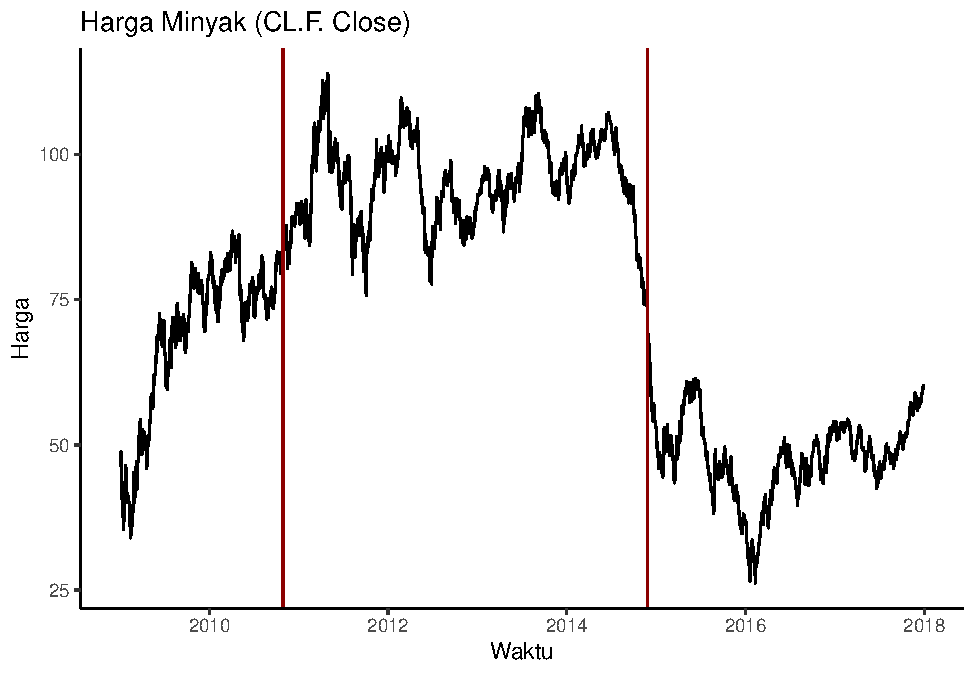
\includegraphics{_main_files/figure-latex/unnamed-chunk-24-1.pdf}

Segmentasi ini akan digunakan sebagai peubah \emph{dummy} yang menjadi input model ARIMAX. Dapat dilihat matriks peubah \emph{dummy} yang akan dipakai, termasuk segmentasi dan efek hari setelah libur:

\begin{Shaded}
\begin{Highlighting}[]
\NormalTok{crudesegmented }\SpecialCharTok{\%\textgreater{}\%} \FunctionTok{select}\NormalTok{(dumMon,dumHol,B1,B2) }\SpecialCharTok{\%\textgreater{}\%} \FunctionTok{head}\NormalTok{(}\DecValTok{10}\NormalTok{) }\SpecialCharTok{\%\textgreater{}\%} 
\NormalTok{  knitr}\SpecialCharTok{::}\FunctionTok{kable}\NormalTok{()}
\end{Highlighting}
\end{Shaded}

\begin{tabular}{r|r|r|r}
\hline
dumMon & dumHol & B1 & B2\\
\hline
0 & 0 & 0 & 0\\
\hline
1 & 0 & 0 & 0\\
\hline
0 & 0 & 0 & 0\\
\hline
0 & 0 & 0 & 0\\
\hline
0 & 0 & 0 & 0\\
\hline
0 & 0 & 0 & 0\\
\hline
1 & 0 & 0 & 0\\
\hline
0 & 0 & 0 & 0\\
\hline
0 & 0 & 0 & 0\\
\hline
0 & 0 & 0 & 0\\
\hline
\end{tabular}

Dapat dilihat bahwa peubah tersebut berkorelasi cukup tinggi dengan harga minyak:

\begin{Shaded}
\begin{Highlighting}[]
\NormalTok{crudesegmented }\SpecialCharTok{\%\textgreater{}\%} \FunctionTok{select}\NormalTok{(B1,B2,fixed) }\SpecialCharTok{\%\textgreater{}\%} \FunctionTok{summarize}\NormalTok{(}\AttributeTok{Break1=}\FunctionTok{cor}\NormalTok{(B1,fixed),}
                                                     \AttributeTok{Break2=}\FunctionTok{cor}\NormalTok{(B2,fixed)) }\SpecialCharTok{\%\textgreater{}\%}
\NormalTok{  knitr}\SpecialCharTok{::}\FunctionTok{kable}\NormalTok{()}
\end{Highlighting}
\end{Shaded}

\begin{tabular}{r|r}
\hline
Break1 & Break2\\
\hline
0.8605528 & -0.8173909\\
\hline
\end{tabular}

Ekstraksi fitur tersebut sepertinya memiliki kemungkinan lebih baik untuk meningkatkan kebaikan model daripada fitur-fitur sebelumnya.

\hypertarget{kestastioneran}{%
\section{Kestastioneran}\label{kestastioneran}}

ACF untuk menunjukkan ketakstasioneran data keseluruhan:

\begin{Shaded}
\begin{Highlighting}[]
\FunctionTok{acf}\NormalTok{(}\FunctionTok{pull}\NormalTok{(crude0917,fixed), }\AttributeTok{plot=}\NormalTok{T)}
\end{Highlighting}
\end{Shaded}

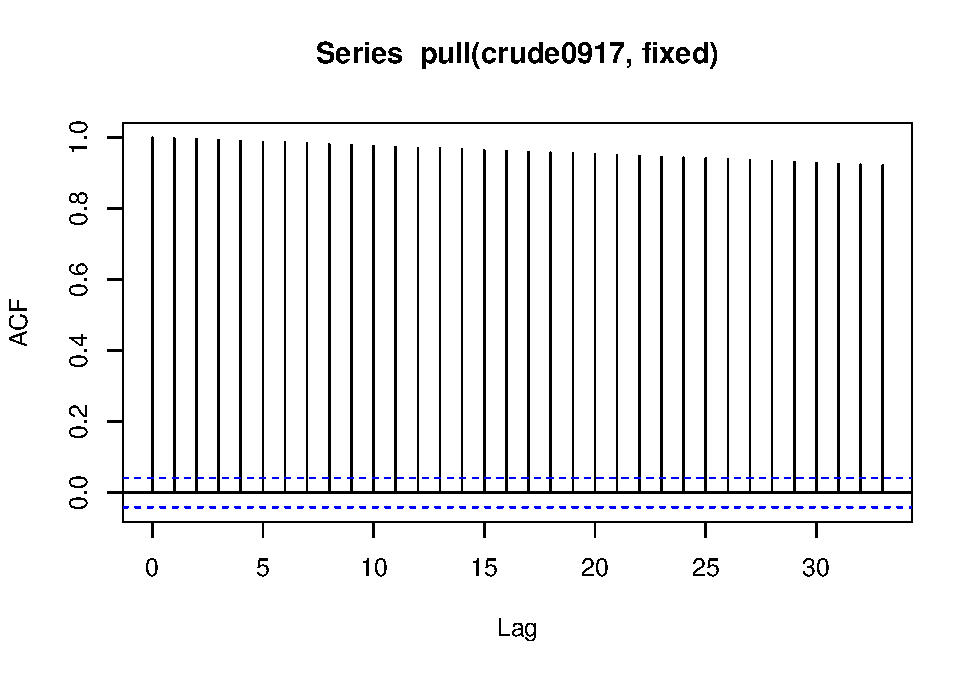
\includegraphics{_main_files/figure-latex/unnamed-chunk-27-1.pdf}

ACF menuruan secara eksponensial hingga data tak stasioner.

\hypertarget{praproses-dan-eksplorasi-data-2017-2022}{%
\chapter{Praproses dan Eksplorasi Data (2017-2022)}\label{praproses-dan-eksplorasi-data-2017-2022}}

Bagian ini akan membahas beberapa hal:

\begin{enumerate}
\def\labelenumi{\arabic{enumi}.}
\tightlist
\item
  Permasalahan interval waktu data
\item
  Latar belakang fluktuasi harga minyak pada tahun 2017-2022
\item
  Ekstraksi peubah \emph{dummy} untuk memodelkan efek COVID-19
\item
  Pola data time series dan kestasioneran
\item
  Identifikasi model.
\end{enumerate}

\hypertarget{interval-waktu-data-1}{%
\section{Interval waktu data}\label{interval-waktu-data-1}}

Dari melihat 10 tanggal pertama yang dicatat di dataset harga minyak:

\begin{Shaded}
\begin{Highlighting}[]
\NormalTok{knitr}\SpecialCharTok{::}\FunctionTok{kable}\NormalTok{(}\FunctionTok{head}\NormalTok{(crudenow,}\AttributeTok{n=}\DecValTok{10}\NormalTok{),}
             \AttributeTok{col.names =} \FunctionTok{c}\NormalTok{(}\StringTok{"Tanggal"}\NormalTok{,}\StringTok{"Harga Penutupan"}\NormalTok{))}
\end{Highlighting}
\end{Shaded}

\begin{tabular}{l|r}
\hline
Tanggal & Harga Penutupan\\
\hline
2017-01-03 & 52.33\\
\hline
2017-01-04 & 53.26\\
\hline
2017-01-05 & 53.76\\
\hline
2017-01-06 & 53.99\\
\hline
2017-01-09 & 51.96\\
\hline
2017-01-10 & 50.82\\
\hline
2017-01-11 & 52.25\\
\hline
2017-01-12 & 53.01\\
\hline
2017-01-13 & 52.37\\
\hline
2017-01-17 & 52.48\\
\hline
\end{tabular}

Terlihat bahwa rentang waktu pengamatan data tidak sama. Misal, tidak ada pengamatan saat 1 Januari 2009 karena ada libur tahun baru. Selain itu, ada lompatan dari 2 Januari 2009 ke 5 Januari 2009. Dalam kata lain, harga minyak tidak diamati pada tanggal 3 dan 4 Januari 2009, yang merupakan akhir minggu (hari Sabtu dan Minggu). Pola yang sama terulang di data deret waktu tersebut bagi akhir minggu dan hari libur lainnya - pasar ditutup sehingga harga minyak tidak ada.

Situasi ini dapat ditangani dengan tiga cara umum:

\begin{enumerate}
\def\labelenumi{\arabic{enumi}.}
\tightlist
\item
  Abaikan rentang waktu harian yang tidak sama. Gunakan \emph{trading days} atau hari kerja sebagai rentang waktu.
\item
  Isi data akhir minggu dan hari libur menggunakan suatu bentuk interpolasi.
\item
  Agregasikan data menjadi data mingguan, bulanan, atau tahunan.
\end{enumerate}

Cara pertama sering dipakai dalam peramalan deret waktu. Walaupun tidak ada data hari libur dan akhir minggu, nilai harian reksadana saham CREF dari tahun 2004 sampai 2006 dimodelkan dengan menggangap data tersebut memiliki rentang waktu yang sama (\protect\hyperlink{ref-cryer_time_2008}{Cryer dan Chan 2008}). Pemodelan harga emas harian dari tahun 1985 sampai 1989 juga hanya menggunakan \emph{trading days}. Dilakukan interpolasi, tetapi hanya untuk data hilang di \emph{trading days} (\protect\hyperlink{ref-fpp2}{Hyndman dan Athanasopoulos 2018}). Peramalan harga minyak (\protect\hyperlink{ref-fouroil}{Elshendy \emph{et al.} 2018}) juga menggunakan data selama 84 hari kerja saja.

Namun, juga ada justifikasi untuk interpolasi data. Interpolasi data dilakukan saat observasi tersebut dianggap memiliki nilai suatu peubah, tetapi tidak dapat diobservasi. Misal, tidak perlu melakukan interpolasi peubah gaji untuk seorang anak karena dia tidak mungkin bekerja. Dalam kasus ini, harga minyak di hari libur mungkin saja memiliki nilai. Pasar saham dan sekuritas sering mengalami \emph{after-hours trading}; saat hal tersebut terjadi, harga berubah (\protect\hyperlink{ref-barclay_price_2015}{Barclay dan Hendershott 2015}). Walaupun begitu, bentuk proses tersebut harus diasumsikan untuk diinterpolasi. Misal, jika menggunakan interpolasi linear, diasumsikan bahwa pergerakan harga dari hari kerja ke hari kerja lainnya di hari libur konstan. Ini belum tentu benar - mungkin saja di hari Sabtu, harga masih naik dari hari Jumat, tetapi harga turun di hari Minggu. Interpolasi linear akan mengasumsikan harga turun di Sabtu dan Minggu. Oleh karena itu, interpolasi akan menghasilkan aproksimasi kasar dari proses \emph{after-hours trading}.

Agregasi data dapat menyelesaikan masalah tersebut karena hasil agregasi dianggap memiliki rentang waktu sama. Misal, mingguan atau bulanan. Agregasi ini harus mengikuti beberapa aturan (\protect\hyperlink{ref-soverflow}{Stefan 2019}). Untuk harga \emph{opening}, akan diambil data harga open dari hari pertama di minggu/bulan tersebut - harga tersebut merupakan harga minyak saat pasar dibuka. Harga \emph{close} diambil dari harga close hari terakhir di minggu/bulan tersebut - harga tersebut merupakan harga minyak saat pasar ditutup. Harga maksimum dan minimum memiliki logika yang mirip.

Namun, agregasi data belum tentu menyelesaikan masalah rentang waktu tak sama. Ada beberapa bulan yang memiliki 28, 30, dan 31 hari. Ini berarti rentang pengamatan satu bulan dapat berarti beberapa jarak waktu yang berbeda. Data mingguan selalu memiliki rentang 7 hari jika data diambil dari hari yang sama di setiap minggu. Dalam kasus ini, ini berarti mengasumsikan data di hari Jumat selalu ada untuk \emph{closing}, atau data hari Senin selalu ada. Mengingat rentang waktu yang cukup lama (8 tahun), kemungkinan besar ada data di hari-hari tersebut yang tidak ada.

Untuk melihat apakah kemungkinan tersebut terjadi, ambil data per minggu. Lalu, kurangkan hari terakhir di minggu tersebut dengan hari terakhir di minggu sebelumnya untuk mendapatkan jarak antarminggu. Akan digunakan fungsi \texttt{ISOweek} dari package dengan nama yang sama (\protect\hyperlink{ref-R-ISOweek}{Block dan Hatto von Hatzfeld 2011}) agar pembagian minggu mengikuti standar ISO 8601. Tabel lalu dimanipulasi menggunakan \texttt{data.table} (\protect\hyperlink{ref-R-data.table}{Dowle dan Srinivasan 2021}), khusunya fungsi shift yang dapat memunculkan lag 1 dari variabel tertentu.

\begin{Shaded}
\begin{Highlighting}[]
\FunctionTok{library}\NormalTok{(ISOweek)}
\FunctionTok{library}\NormalTok{(data.table)}

\NormalTok{weeklyCrude}\OtherTok{\textless{}{-}}\NormalTok{crudenow[,Week}\SpecialCharTok{:}\ErrorTok{=}\FunctionTok{ISOweek}\NormalTok{(X)}
\NormalTok{         ][,.(}\AttributeTok{Date=}\FunctionTok{last}\NormalTok{(X),}
            \AttributeTok{Close=}\FunctionTok{last}\NormalTok{(}\StringTok{\textasciigrave{}}\AttributeTok{CL=F.Close}\StringTok{\textasciigrave{}}\NormalTok{)),by}\OtherTok{=}\FunctionTok{list}\NormalTok{(Week)}
\NormalTok{           ][,Dist}\SpecialCharTok{:}\ErrorTok{=}\NormalTok{Date}\SpecialCharTok{{-}}\FunctionTok{shift}\NormalTok{(Date)]}
\end{Highlighting}
\end{Shaded}

Tidak semua minggu memiliki jarak 7 hari. Ada beberapa minggu dengan jarak 6 dan 8 hari:

\begin{Shaded}
\begin{Highlighting}[]
\NormalTok{knitr}\SpecialCharTok{::}\FunctionTok{kable}\NormalTok{(weeklyCrude[,.(}\AttributeTok{count=}\NormalTok{.N),}\AttributeTok{by=}\NormalTok{Dist], }\AttributeTok{col.names =} \FunctionTok{c}\NormalTok{(}\StringTok{"Jarak"}\NormalTok{,}
                                                              \StringTok{"Jumlah"}\NormalTok{))}
\end{Highlighting}
\end{Shaded}

\begin{tabular}{l|r}
\hline
Jarak & Jumlah\\
\hline
NA days & 1\\
\hline
7 days & 258\\
\hline
6 days & 8\\
\hline
8 days & 8\\
\hline
\end{tabular}

Dapat diekstraksi peubah \emph{dummy} dari minggu-minggu dengan jarak lebih dari 7 hari untuk memodelkan efek minggu-minggu tersebut.

\begin{Shaded}
\begin{Highlighting}[]
\NormalTok{weeklyCrude[,Dist}\SpecialCharTok{:}\ErrorTok{=}\FunctionTok{na.fill}\NormalTok{(Dist,}\AttributeTok{type=}\StringTok{"const"}\NormalTok{,}\AttributeTok{fill=}\FunctionTok{as.Date}\NormalTok{(}\DecValTok{7}\NormalTok{))}
\NormalTok{         ][,}\StringTok{\textasciigrave{}}\AttributeTok{:=}\StringTok{\textasciigrave{}}\NormalTok{(}\StringTok{"6DW"}\OtherTok{=}\FunctionTok{ifelse}\NormalTok{(Dist}\SpecialCharTok{==}\DecValTok{6}\NormalTok{,}\DecValTok{1}\NormalTok{,}\DecValTok{0}\NormalTok{),}
               \StringTok{"8DW"}\OtherTok{=}\FunctionTok{ifelse}\NormalTok{(Dist}\SpecialCharTok{==}\DecValTok{8}\NormalTok{,}\DecValTok{1}\NormalTok{,}\DecValTok{0}\NormalTok{))]}
\end{Highlighting}
\end{Shaded}

Peubah tersebut nantinya dapat digunakan dalam pemodelan. Namun, sepertinya baik \emph{dummy} dengan untuk minggu periode 6 hari dan 8 hari tidak berkorelasi terlalu besar dengan harga minyak saat penutupan pasar:

\begin{Shaded}
\begin{Highlighting}[]
\NormalTok{knitr}\SpecialCharTok{::}\FunctionTok{kable}\NormalTok{(}\FunctionTok{t}\NormalTok{(}\FunctionTok{c}\NormalTok{(}\FunctionTok{cor}\NormalTok{(weeklyCrude}\SpecialCharTok{$}\StringTok{\textasciigrave{}}\AttributeTok{6DW}\StringTok{\textasciigrave{}}\NormalTok{,weeklyCrude}\SpecialCharTok{$}\NormalTok{Close,}\AttributeTok{method=}\StringTok{"spearman"}\NormalTok{),}
               \FunctionTok{cor}\NormalTok{(weeklyCrude}\SpecialCharTok{$}\StringTok{\textasciigrave{}}\AttributeTok{8DW}\StringTok{\textasciigrave{}}\NormalTok{,weeklyCrude}\SpecialCharTok{$}\NormalTok{Close,}\AttributeTok{method=}\StringTok{"spearman"}\NormalTok{))),}
               \AttributeTok{col.names=}\FunctionTok{c}\NormalTok{(}\StringTok{"6 Hari"}\NormalTok{,}\StringTok{"8 hari"}\NormalTok{),}
               \AttributeTok{row.names=}\NormalTok{F)}
\end{Highlighting}
\end{Shaded}

\begin{tabular}{r|r}
\hline
6 Hari & 8 hari\\
\hline
-0.029709 & -0.0391122\\
\hline
\end{tabular}

\hypertarget{plot-data}{%
\section{Plot data}\label{plot-data}}

Untuk melihat jenis data yang dihadapi, dapat di-plot data deret waktu mingguan harga minyak dari tahun 2017-2022 dengan ggplot2 (\protect\hyperlink{ref-R-ggplot2}{Wickham \emph{et al.} 2021}):

\begin{Shaded}
\begin{Highlighting}[]
\FunctionTok{ggplot}\NormalTok{(}\FunctionTok{aes}\NormalTok{(}\AttributeTok{x=}\NormalTok{Date, }\AttributeTok{y=}\NormalTok{Close),}\AttributeTok{data=}\NormalTok{weeklyCrude) }\SpecialCharTok{+}
  \FunctionTok{geom\_line}\NormalTok{()}\SpecialCharTok{+}\FunctionTok{ggtitle}\NormalTok{(}\StringTok{"Harga Minyak (CL.F. Close) {-} USD/Barrel"}\NormalTok{)}\SpecialCharTok{+}
  \FunctionTok{xlab}\NormalTok{(}\StringTok{"Waktu"}\NormalTok{)}\SpecialCharTok{+}\FunctionTok{ylab}\NormalTok{(}\StringTok{" "}\NormalTok{)}\SpecialCharTok{+}\FunctionTok{theme\_bw}\NormalTok{()}
\end{Highlighting}
\end{Shaded}

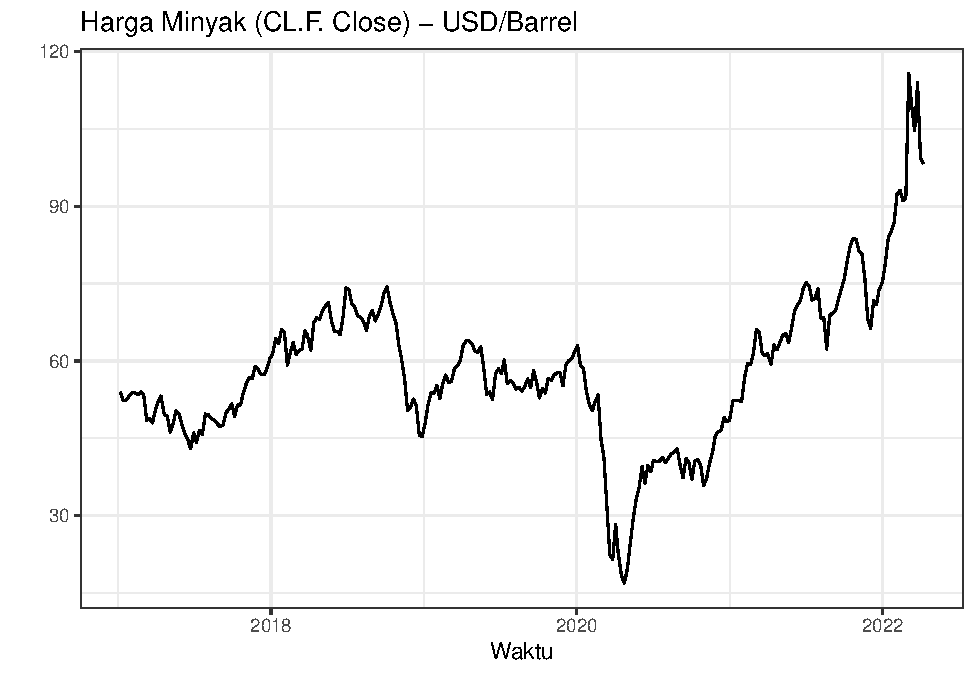
\includegraphics{_main_files/figure-latex/unnamed-chunk-33-1.pdf}

Data jelas tidak stasioner.

\hypertarget{latar-belakang-1}{%
\section{Latar Belakang}\label{latar-belakang-1}}

\begin{Shaded}
\begin{Highlighting}[]
\NormalTok{cbbPalette }\OtherTok{\textless{}{-}} \FunctionTok{c}\NormalTok{(}\StringTok{"\#E69F00"}\NormalTok{, }\StringTok{"\#56B4E9"}\NormalTok{, }\StringTok{"\#D3D3D3"}\NormalTok{, }\StringTok{"\#009E73"}\NormalTok{, }\StringTok{"\#CC79A7"}\NormalTok{)}
\NormalTok{highlightPalette}\OtherTok{\textless{}{-}}\FunctionTok{c}\NormalTok{(}\StringTok{"\#D3D3D3"}\NormalTok{,}\StringTok{"\#00008b"}\NormalTok{)}

\NormalTok{weeklyCrude[,}\StringTok{"2017 {-} Siklik"}\SpecialCharTok{:}\ErrorTok{=}\FunctionTok{ifelse}\NormalTok{(Date}\SpecialCharTok{\textless{}=}\FunctionTok{as.Date}\NormalTok{(}\StringTok{"2017{-}11{-}10"}\NormalTok{),T,F)]}
\FunctionTok{ggplot}\NormalTok{(}\FunctionTok{aes}\NormalTok{(}\AttributeTok{x=}\NormalTok{Date, }\AttributeTok{y=}\NormalTok{Close),}
       \AttributeTok{data=}\NormalTok{weeklyCrude)}\SpecialCharTok{+}
  \FunctionTok{geom\_line}\NormalTok{(}\FunctionTok{aes}\NormalTok{(}\AttributeTok{color=}\StringTok{\textasciigrave{}}\AttributeTok{2017 {-} Siklik}\StringTok{\textasciigrave{}}\NormalTok{))}\SpecialCharTok{+}\FunctionTok{scale\_color\_manual}\NormalTok{(}\AttributeTok{values=}\NormalTok{highlightPalette)}\SpecialCharTok{+}
  \FunctionTok{ggtitle}\NormalTok{(}\StringTok{"Harga Minyak (CL.F. Close) {-} USD/Barrel"}\NormalTok{)}\SpecialCharTok{+}\FunctionTok{xlab}\NormalTok{(}\StringTok{"Waktu"}\NormalTok{)}\SpecialCharTok{+}\FunctionTok{ylab}\NormalTok{(}\StringTok{" "}\NormalTok{)}\SpecialCharTok{+}
  \FunctionTok{theme\_bw}\NormalTok{()}
\end{Highlighting}
\end{Shaded}

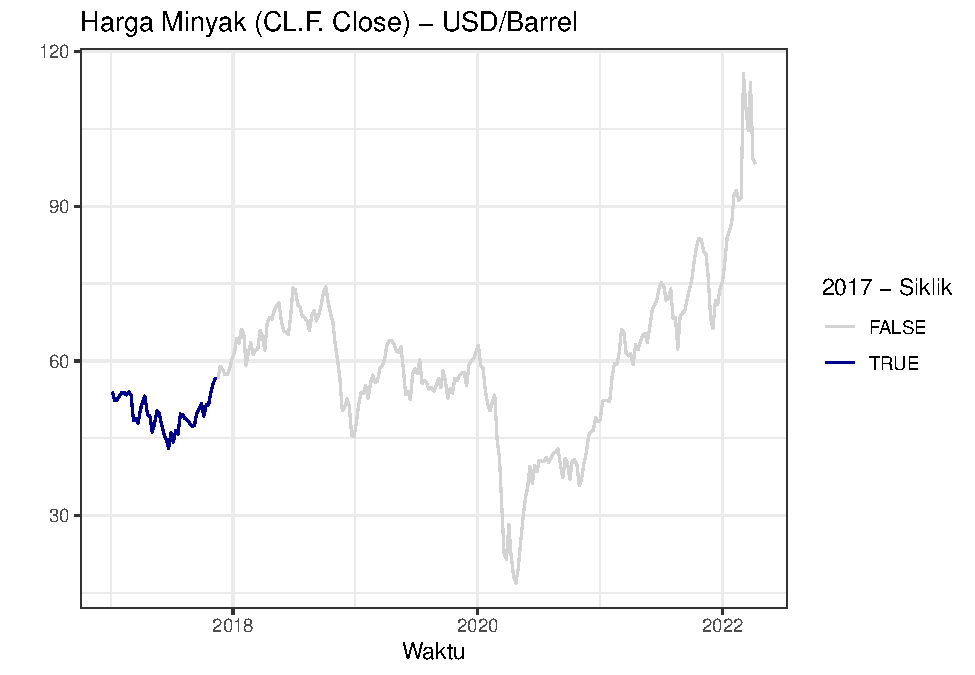
\includegraphics{_main_files/figure-latex/unnamed-chunk-34-1.pdf}

Di awal tahun 2017, harga minyak menurun karena komitmen produsen minyak di OPEC untuk memotong produksi minyak diragukan. Selain itu, turunnya volume ekspor Tiongkok menandakan kemungkinan lemahnya permintaan untuk minyak mentah (\protect\hyperlink{ref-reu_oil_2017}{Kumar 2017 Jan}). Namun, harga minyak sedikit naik di akhir Januari 2017 karena melemahnya dolar Amerika Serikat - minyak dibeli menggunakan dolar Amerika Serikat, sehingga dolar yang lebih lemah berarti negara pengimpor minyak dapat membeli lebih banyak minyak mentah yang meningkatkan permintaan (\protect\hyperlink{ref-reu_oil_2017-1}{Gloystein 2017 Jan}).

Walaupun terdapat fenomena tersebut, pasokan minyak masih meningkat sehingga harga minyak turun sampai Maret. Arab Saudi berjanji untuk menurunkan produksi di bulan April, tetapi produksi minyak negara OPEC justru meningkat di bulan Juni sampai harga minyak mencapai titik terendahnya (\protect\hyperlink{ref-reu_oil_2017-4}{Gloystein 2017 Jun}). Janji OPEC untuk menurunkan produksi minyak dipenuhi di paruh kedua 2017 dan permintaan meningkat. Oleh karena itu, harga minyak meningkat sampai pulih ke level sebelum bulan Juni di bulan November (\protect\hyperlink{ref-reu_oil_2017-6}{Gloystein 2017 Des}).

Secara umum, periode ini ditandakan dengan siklus. Negara OPEC berjanji menurunkan produksi (yang meningkatkan harga), tetapi produksi sebenarnaya masih tinggi (yang menurunkan harga) sehingga harga turun lalu naik.

\begin{Shaded}
\begin{Highlighting}[]
\NormalTok{weeklyCrude[,}\StringTok{"Awal 2018 {-} harga naik"}\SpecialCharTok{:}\ErrorTok{=}\FunctionTok{ifelse}\NormalTok{(Date}\SpecialCharTok{\textgreater{}=}\FunctionTok{as.Date}\NormalTok{(}\StringTok{"2017{-}11{-}10"}\NormalTok{) }\SpecialCharTok{\&}\NormalTok{ Date}\SpecialCharTok{\textless{}=}\FunctionTok{as.Date}\NormalTok{(}\StringTok{"2018{-}10{-}10"}\NormalTok{),T,F)]}
\FunctionTok{ggplot}\NormalTok{(}\FunctionTok{aes}\NormalTok{(}\AttributeTok{x=}\NormalTok{Date, }\AttributeTok{y=}\NormalTok{Close),}
       \AttributeTok{data=}\NormalTok{weeklyCrude)}\SpecialCharTok{+}
  \FunctionTok{geom\_line}\NormalTok{(}\FunctionTok{aes}\NormalTok{(}\AttributeTok{color=}\StringTok{\textasciigrave{}}\AttributeTok{Awal 2018 {-} harga naik}\StringTok{\textasciigrave{}}\NormalTok{))}\SpecialCharTok{+}\FunctionTok{scale\_color\_manual}\NormalTok{(}\AttributeTok{values=}\NormalTok{highlightPalette)}\SpecialCharTok{+}
  \FunctionTok{ggtitle}\NormalTok{(}\StringTok{"Harga Minyak (CL.F. Close) {-} USD/Barrel"}\NormalTok{)}\SpecialCharTok{+}\FunctionTok{xlab}\NormalTok{(}\StringTok{"Waktu"}\NormalTok{)}\SpecialCharTok{+}\FunctionTok{ylab}\NormalTok{(}\StringTok{" "}\NormalTok{)}\SpecialCharTok{+}
  \FunctionTok{theme\_bw}\NormalTok{()}
\end{Highlighting}
\end{Shaded}

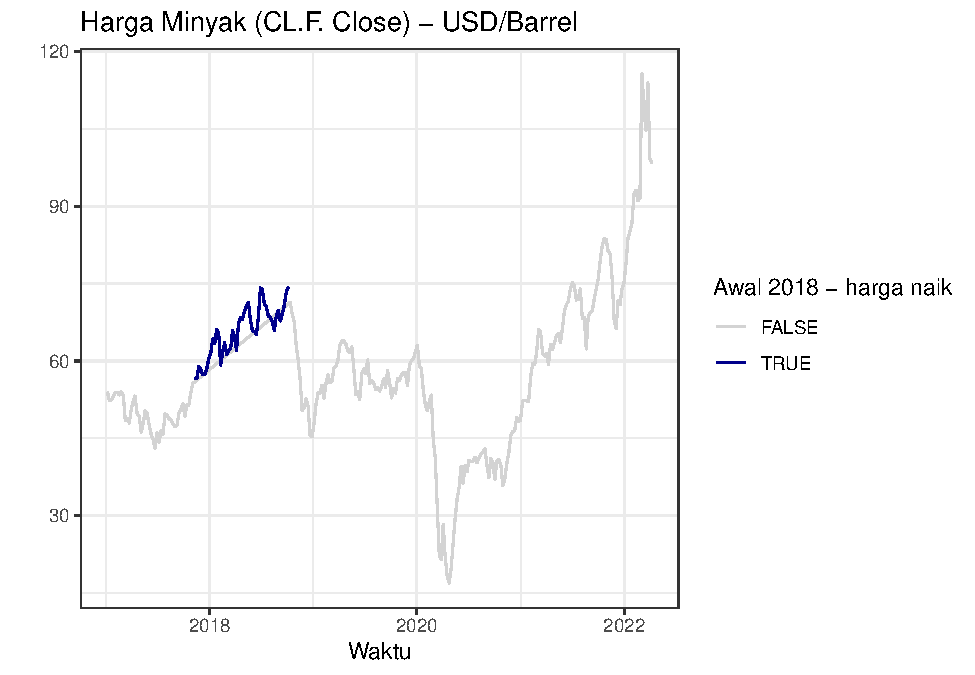
\includegraphics{_main_files/figure-latex/unnamed-chunk-35-1.pdf}

Harga minyak naik di akhir tahun 2017 sampai triwulan ketiga 2018. Selain turunnya produksi minyak oleh OPEC, terjadi gangguan pipa minyak di Libya dan Rusia yang menganggu distribusi minyak. Di awal Januari 2018, rendahnya pasokan minyak dunia meningkatkan harga. Walaupun terjadi sedikit penurunan karena Amerika Serikat berencana meningkatkan produksi (\protect\hyperlink{ref-reu_oil_2018}{Gloystein 2018 Jan}), negara-negara OPEC masih memotong produksi karena ingin meningkatkan harga minyak. Pada Maret sampai Mei 2018, harga minyak naik karena ketidakstabilan di Suriah, kemungkinan pembatasan impor minyak dari Iran, dan rendahnya produksi minyak OPEC dan Venezuela.

\begin{Shaded}
\begin{Highlighting}[]
\NormalTok{weeklyCrude[,}\StringTok{"Akhir 2018 {-} harga turun"}\SpecialCharTok{:}\ErrorTok{=}
              \FunctionTok{ifelse}\NormalTok{(Date}\SpecialCharTok{\textgreater{}=}\FunctionTok{as.Date}\NormalTok{(}\StringTok{"2018{-}10{-}10"}\NormalTok{) }\SpecialCharTok{\&}\NormalTok{ Date}\SpecialCharTok{\textless{}=}\FunctionTok{as.Date}\NormalTok{(}\StringTok{"2018{-}12{-}31"}\NormalTok{),T,F)]}
\FunctionTok{ggplot}\NormalTok{(}\FunctionTok{aes}\NormalTok{(}\AttributeTok{x=}\NormalTok{Date, }\AttributeTok{y=}\NormalTok{Close),}
       \AttributeTok{data=}\NormalTok{weeklyCrude)}\SpecialCharTok{+}
  \FunctionTok{geom\_line}\NormalTok{(}\FunctionTok{aes}\NormalTok{(}\AttributeTok{color=}\StringTok{\textasciigrave{}}\AttributeTok{Akhir 2018 {-} harga turun}\StringTok{\textasciigrave{}}\NormalTok{))}\SpecialCharTok{+}\FunctionTok{scale\_color\_manual}\NormalTok{(}\AttributeTok{values=}\NormalTok{highlightPalette)}\SpecialCharTok{+}
  \FunctionTok{ggtitle}\NormalTok{(}\StringTok{"Harga Minyak (CL.F. Close) {-} USD/Barrel"}\NormalTok{)}\SpecialCharTok{+}\FunctionTok{xlab}\NormalTok{(}\StringTok{"Waktu"}\NormalTok{)}\SpecialCharTok{+}\FunctionTok{ylab}\NormalTok{(}\StringTok{" "}\NormalTok{)}\SpecialCharTok{+}
  \FunctionTok{theme\_bw}\NormalTok{()}
\end{Highlighting}
\end{Shaded}

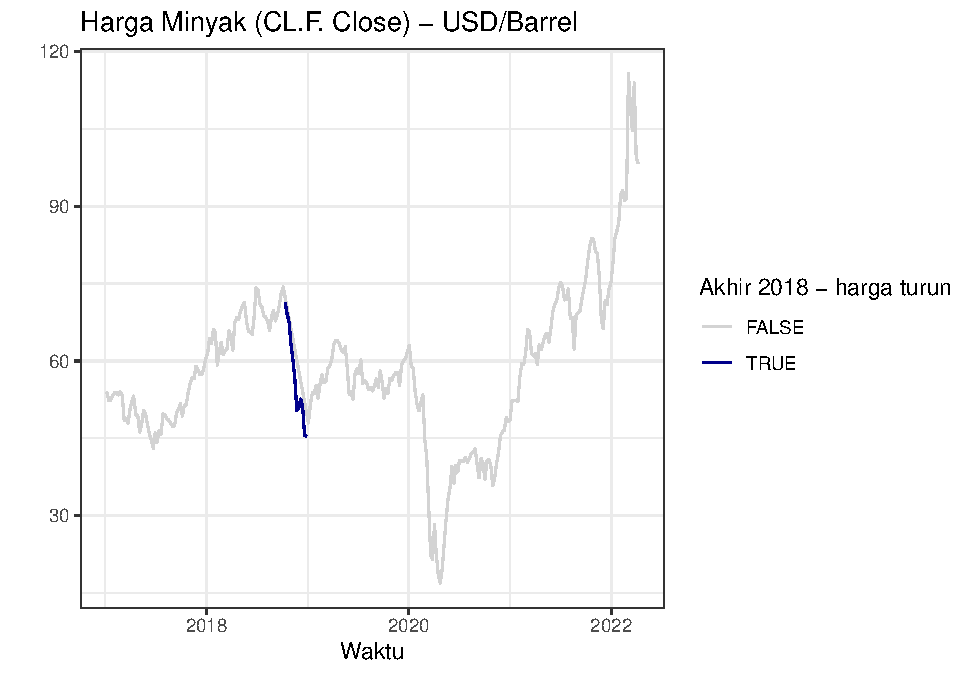
\includegraphics{_main_files/figure-latex/unnamed-chunk-36-1.pdf}

Harga minyak turun drastis di akhir tahun 2018. Rusia dan Arab Saudi mengumumkan peningkatan produksi untuk menggantikan minyak Iran, pemerintah Amerika Serikat memberi dispensasi ke beberapa perusahaan Iran (\protect\hyperlink{ref-woolich_sanctions_nodate}{Woolich \emph{et al.} 2018}), dan produksi \emph{shale oil} as meningkat. Dari sisi penawaran, pasokan minyak meningkat yang menurunkan harga (\protect\hyperlink{ref-dichristopher_us_2018}{DiChristopher 2018 Des}).

\begin{Shaded}
\begin{Highlighting}[]
\NormalTok{weeklyCrude[, }\StringTok{"Pra{-}COVID"}\SpecialCharTok{:}\ErrorTok{=}
            \FunctionTok{ifelse}\NormalTok{(Date}\SpecialCharTok{\textgreater{}=}\FunctionTok{as.Date}\NormalTok{(}\StringTok{"2019{-}01{-}01"}\NormalTok{) }\SpecialCharTok{\&}\NormalTok{ Date}\SpecialCharTok{\textless{}=}\FunctionTok{as.Date}\NormalTok{(}\StringTok{"2020{-}02{-}03"}\NormalTok{),T,F)]}
\FunctionTok{ggplot}\NormalTok{(}\FunctionTok{aes}\NormalTok{(}\AttributeTok{x=}\NormalTok{Date, }\AttributeTok{y=}\NormalTok{Close),}
       \AttributeTok{data=}\NormalTok{weeklyCrude)}\SpecialCharTok{+}
  \FunctionTok{geom\_line}\NormalTok{(}\FunctionTok{aes}\NormalTok{(}\AttributeTok{color=}\StringTok{\textasciigrave{}}\AttributeTok{Pra{-}COVID}\StringTok{\textasciigrave{}}\NormalTok{))}\SpecialCharTok{+}\FunctionTok{scale\_color\_manual}\NormalTok{(}\AttributeTok{values=}\NormalTok{highlightPalette)}\SpecialCharTok{+}
  \FunctionTok{ggtitle}\NormalTok{(}\StringTok{"Harga Minyak (CL.F. Close) {-} USD/Barrel"}\NormalTok{)}\SpecialCharTok{+}\FunctionTok{xlab}\NormalTok{(}\StringTok{"Waktu"}\NormalTok{)}\SpecialCharTok{+}\FunctionTok{ylab}\NormalTok{(}\StringTok{" "}\NormalTok{)}\SpecialCharTok{+}
  \FunctionTok{theme\_bw}\NormalTok{()}
\end{Highlighting}
\end{Shaded}

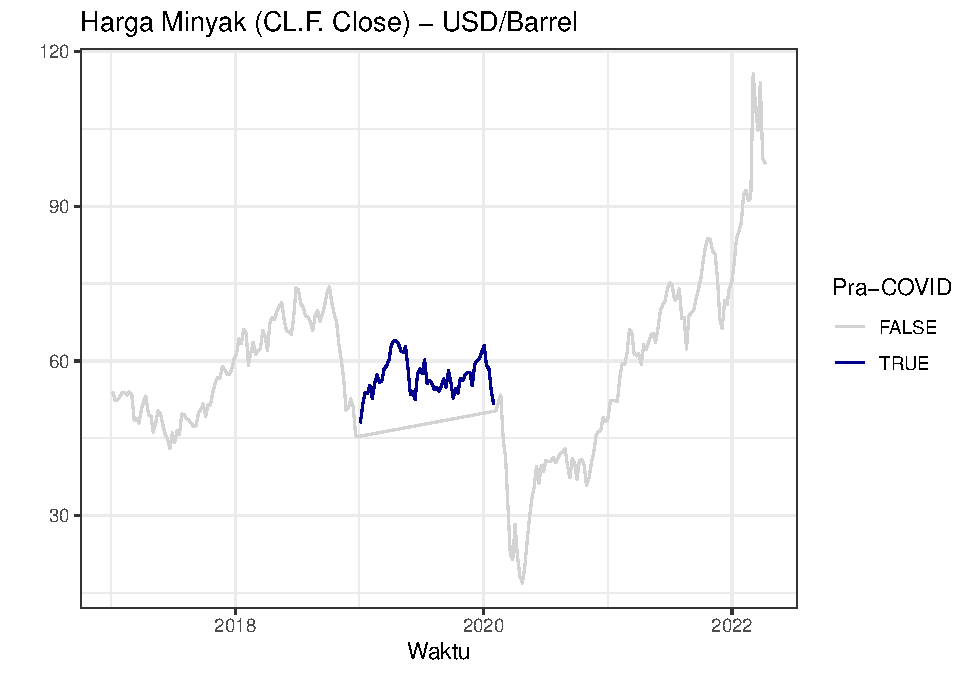
\includegraphics{_main_files/figure-latex/unnamed-chunk-37-1.pdf}

Tahun 2019 diawali dengan peningkatan harga minyak karena penurunan produksi dari Arab Saudi dan sanksi kepada Venezuela. Terdapat penurunan harga di bulan Februari karena melambatnya pertumbuhan ekonomi di Amerika Serikat, yang menghasilkan sedikit fluktuasi naik-turun, tetapi harga minyak tetap naik karena dispensasi ke eksportir minyak Iran berakhir dan pembatasan perdagangan minyak diberlakukan (\protect\hyperlink{ref-welle_wwwdwcom_us_nodate}{2019}). Namun, setelah mencapai puncak di bulan April, harga minyak turun di bulan Mei saat Amerika Serikat mengumumkan perang dagang dengan Tiongkok (\protect\hyperlink{ref-reu_oil_2019}{Kumar 2019 Agu}). Harga kembali naik di bulan Juni setelah Iran menjatuhkan \emph{drone} Amerika Serikat, yang meningkatkan ketidakstabilan di Timur Tengah. Pengumuman tarif baru dalam perang dagang oleh Amerika Serikat menurunkan kembali harga minyak, tetapi ekspektasi penurunan produksi oleh OPEC meningkatkan harga minyak di November 2019.

Secara umum, fluktuasi naik-turun terjadi karena tekanan perang dagang (yang menurunkan harga karena menurunkan permintaan minyak) dan tekanan dari OPEC serta ketidakstabilan Timur Tengah yag meningkatkan harga minyak.

\begin{Shaded}
\begin{Highlighting}[]
\NormalTok{weeklyCrude[,}\StringTok{"COVID"}\SpecialCharTok{:}\ErrorTok{=}
              \FunctionTok{ifelse}\NormalTok{(Date}\SpecialCharTok{\textgreater{}=}\FunctionTok{as.Date}\NormalTok{(}\StringTok{"2020{-}02{-}03"}\NormalTok{) }\SpecialCharTok{\&}\NormalTok{ Date}\SpecialCharTok{\textless{}=}\FunctionTok{as.Date}\NormalTok{(}\StringTok{"2020{-}04{-}30"}\NormalTok{),T,F)]}
\FunctionTok{ggplot}\NormalTok{(}\FunctionTok{aes}\NormalTok{(}\AttributeTok{x=}\NormalTok{Date, }\AttributeTok{y=}\NormalTok{Close),}
       \AttributeTok{data=}\NormalTok{weeklyCrude)}\SpecialCharTok{+}
  \FunctionTok{geom\_line}\NormalTok{(}\FunctionTok{aes}\NormalTok{(}\AttributeTok{color=}\StringTok{\textasciigrave{}}\AttributeTok{COVID}\StringTok{\textasciigrave{}}\NormalTok{))}\SpecialCharTok{+}\FunctionTok{scale\_color\_manual}\NormalTok{(}\AttributeTok{values=}\NormalTok{highlightPalette)}\SpecialCharTok{+}
  \FunctionTok{ggtitle}\NormalTok{(}\StringTok{"Harga Minyak (CL.F. Close) {-} USD/Barrel"}\NormalTok{)}\SpecialCharTok{+}\FunctionTok{xlab}\NormalTok{(}\StringTok{"Waktu"}\NormalTok{)}\SpecialCharTok{+}\FunctionTok{ylab}\NormalTok{(}\StringTok{" "}\NormalTok{)}\SpecialCharTok{+}
  \FunctionTok{theme\_bw}\NormalTok{()}
\end{Highlighting}
\end{Shaded}

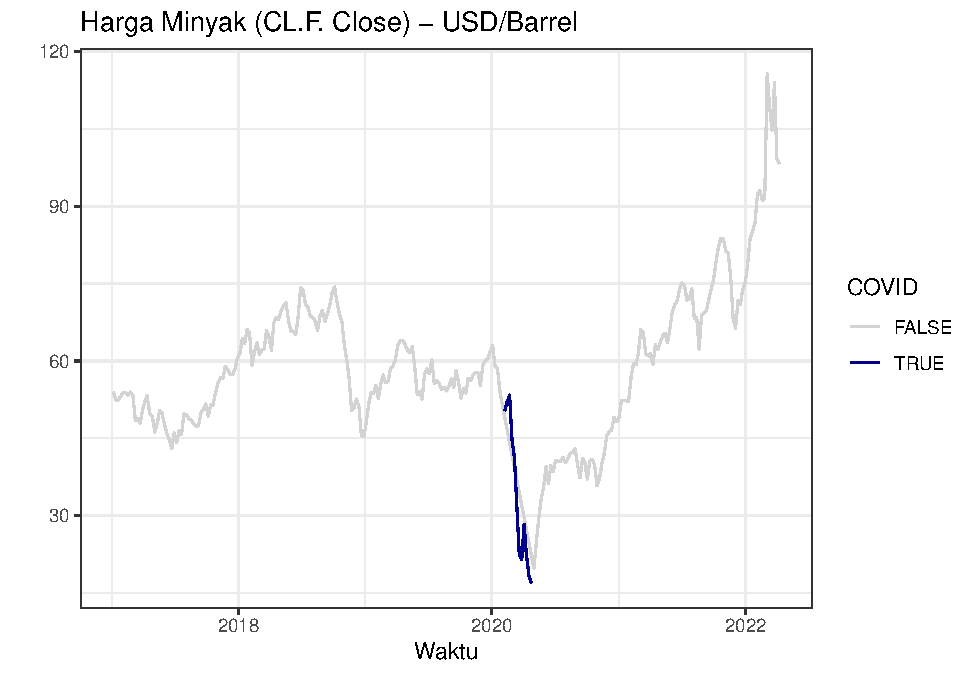
\includegraphics{_main_files/figure-latex/unnamed-chunk-38-1.pdf}

Harga minyak dunia terjun bebas dari Februari sampai April 2020. Pandemi COVID-19 mengurangi aktivitas ekonomi sehingga permintaan minyak berkurang. Karena itu, negara-negara OPEC setuju untuk mengurangi produksi, kecuali Rusia. Terjadi perang harga minyak antara Arab Saudi dan Rusia. Arab Saudi meningkatkan produksi dan memberikan diskon harga minyak, sampai minyak turun drastis (\protect\hyperlink{ref-calhoun_saudirussia_nodate}{Calhoun 2020}). Akhirnya, tekanan dari Amerika Serikat ke Arab Saudi (dan penurunan devisa Arab Saudi dan Rusia saat harga minyak rendah) membuat kedua negara setuju untuk memotong produksi. Namun, harga masih turun di akhir April sampai menjadi negatif karena biaya menyimpan minyak lebih mahal dari harga jualnya (\protect\hyperlink{ref-lw_oil_2020}{Mills 2020 Apr}).

\begin{Shaded}
\begin{Highlighting}[]
\NormalTok{weeklyCrude[,}\StringTok{"Pemulihan"}\SpecialCharTok{:}\ErrorTok{=}
              \FunctionTok{ifelse}\NormalTok{(Date}\SpecialCharTok{\textgreater{}=}\FunctionTok{as.Date}\NormalTok{(}\StringTok{"2020{-}04{-}30"}\NormalTok{) }\SpecialCharTok{\&}\NormalTok{ Date}\SpecialCharTok{\textless{}=}\FunctionTok{as.Date}\NormalTok{(}\StringTok{"2020{-}10{-}24"}\NormalTok{),T,F)]}
\FunctionTok{ggplot}\NormalTok{(}\FunctionTok{aes}\NormalTok{(}\AttributeTok{x=}\NormalTok{Date, }\AttributeTok{y=}\NormalTok{Close),}
       \AttributeTok{data=}\NormalTok{weeklyCrude)}\SpecialCharTok{+}
  \FunctionTok{geom\_line}\NormalTok{(}\FunctionTok{aes}\NormalTok{(}\AttributeTok{color=}\StringTok{\textasciigrave{}}\AttributeTok{Pemulihan}\StringTok{\textasciigrave{}}\NormalTok{))}\SpecialCharTok{+}\FunctionTok{scale\_color\_manual}\NormalTok{(}\AttributeTok{values=}\NormalTok{highlightPalette)}\SpecialCharTok{+}
  \FunctionTok{ggtitle}\NormalTok{(}\StringTok{"Harga Minyak (CL.F. Close) {-} USD/Barrel"}\NormalTok{)}\SpecialCharTok{+}\FunctionTok{xlab}\NormalTok{(}\StringTok{"Waktu"}\NormalTok{)}\SpecialCharTok{+}\FunctionTok{ylab}\NormalTok{(}\StringTok{" "}\NormalTok{)}\SpecialCharTok{+}
  \FunctionTok{theme\_bw}\NormalTok{()}
\end{Highlighting}
\end{Shaded}

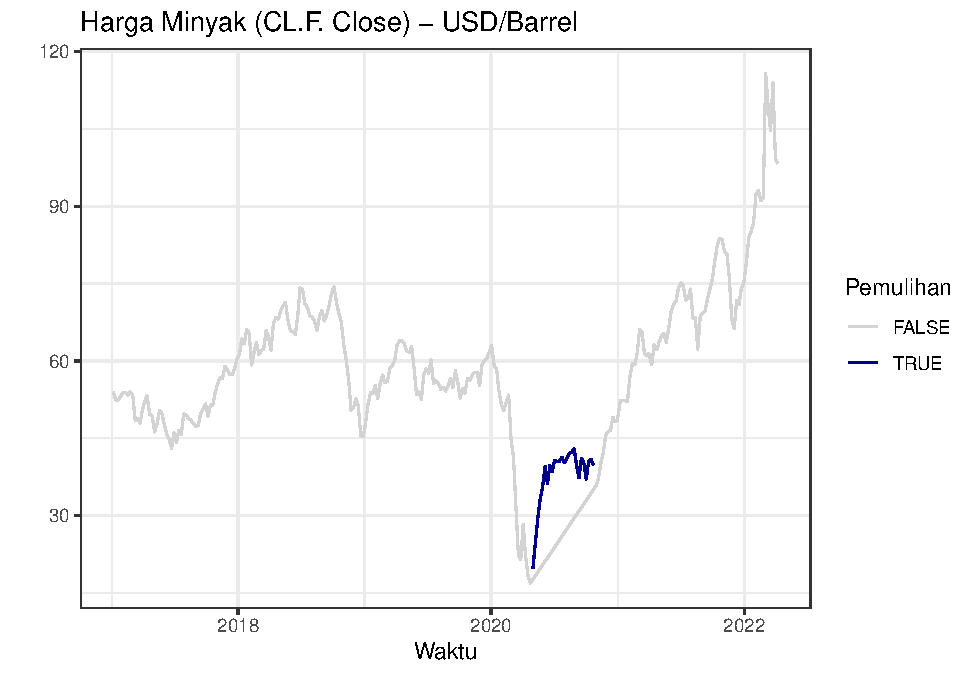
\includegraphics{_main_files/figure-latex/unnamed-chunk-39-1.pdf}

Setelah bulan April, penurunan produksi minyak OPEC dan Amerika Serikat mulai memiliki efek dan harga minyak kembali meningkat. Di bulan Juli harga minyak turun sedikit karena menguatnya dolar (sehingga pengimpor minyak susah membeli minyak), rendahnya permintaan, dan pasokan Amerika Serikat yang lebih tinggi dari harapan. Berita mengenai Presiden Amerika Serikat pada bulan Oktober, Donald Trump, yang terkena COVID juga menurunkan harga minyak. Namun, fluktuasi tersebut relatif kecil dibandingkan fluktuasi-fluktuasi yang terjadi saat awal COVID. Berita mengenai vaksin COVID di akhir 2020 (\protect\hyperlink{ref-pfizer_2020}{Pfizer 2020 Nov}) meningkatkan kepercayaan bahwa ekonomi dunia akan kembali pulih, dan harga minyak mulai naik.

\begin{Shaded}
\begin{Highlighting}[]
\NormalTok{weeklyCrude[,}\StringTok{"Vaksin, Varian"}\SpecialCharTok{:}\ErrorTok{=}
              \FunctionTok{ifelse}\NormalTok{(Date}\SpecialCharTok{\textgreater{}=}\FunctionTok{as.Date}\NormalTok{(}\StringTok{"2020{-}10{-}24"}\NormalTok{) }\SpecialCharTok{\&}\NormalTok{ Date}\SpecialCharTok{\textless{}=}\FunctionTok{as.Date}\NormalTok{(}\StringTok{"2021{-}02{-}13"}\NormalTok{),}
                     \StringTok{"Vaksinasi"}\NormalTok{,}
              \FunctionTok{ifelse}\NormalTok{(Date}\SpecialCharTok{\textgreater{}=}\FunctionTok{as.Date}\NormalTok{(}\StringTok{"2021{-}02{-}02"}\NormalTok{) }\SpecialCharTok{\&}\NormalTok{ Date}\SpecialCharTok{\textless{}=}\FunctionTok{as.Date}\NormalTok{(}\StringTok{"2021{-}05{-}07"}\NormalTok{),}
                     \StringTok{"Alpha"}\NormalTok{,}
              \FunctionTok{ifelse}\NormalTok{(Date}\SpecialCharTok{\textgreater{}=}\FunctionTok{as.Date}\NormalTok{(}\StringTok{"2021{-}05{-}07"}\NormalTok{) }\SpecialCharTok{\&}\NormalTok{ Date}\SpecialCharTok{\textless{}=}\FunctionTok{as.Date}\NormalTok{(}\StringTok{"2021{-}09{-}01"}\NormalTok{),}
                     \StringTok{"Delta"}\NormalTok{,}
              \FunctionTok{ifelse}\NormalTok{(Date}\SpecialCharTok{\textgreater{}=}\FunctionTok{as.Date}\NormalTok{(}\StringTok{"2021{-}09{-}01"}\NormalTok{) }\SpecialCharTok{\&}\NormalTok{ Date}\SpecialCharTok{\textless{}=}\FunctionTok{as.Date}\NormalTok{(}\StringTok{"2021{-}12{-}01"}\NormalTok{),}
                     \StringTok{"Omicron"}\NormalTok{,}\StringTok{"Lainnya"}\NormalTok{))))]}
\FunctionTok{ggplot}\NormalTok{(}\FunctionTok{aes}\NormalTok{(}\AttributeTok{x=}\NormalTok{Date, }\AttributeTok{y=}\NormalTok{Close),}
       \AttributeTok{data=}\NormalTok{weeklyCrude)}\SpecialCharTok{+}
  \FunctionTok{geom\_line}\NormalTok{(}\FunctionTok{aes}\NormalTok{(}\AttributeTok{color=}\StringTok{\textasciigrave{}}\AttributeTok{Vaksin, Varian}\StringTok{\textasciigrave{}}\NormalTok{))}\SpecialCharTok{+}\FunctionTok{scale\_color\_manual}\NormalTok{(}\AttributeTok{values=}\NormalTok{cbbPalette)}\SpecialCharTok{+}
  \FunctionTok{ggtitle}\NormalTok{(}\StringTok{"Harga Minyak (CL.F. Close) {-} USD/Barrel"}\NormalTok{)}\SpecialCharTok{+}\FunctionTok{xlab}\NormalTok{(}\StringTok{"Waktu"}\NormalTok{)}\SpecialCharTok{+}\FunctionTok{ylab}\NormalTok{(}\StringTok{" "}\NormalTok{)}\SpecialCharTok{+}
  \FunctionTok{theme\_bw}\NormalTok{()}
\end{Highlighting}
\end{Shaded}

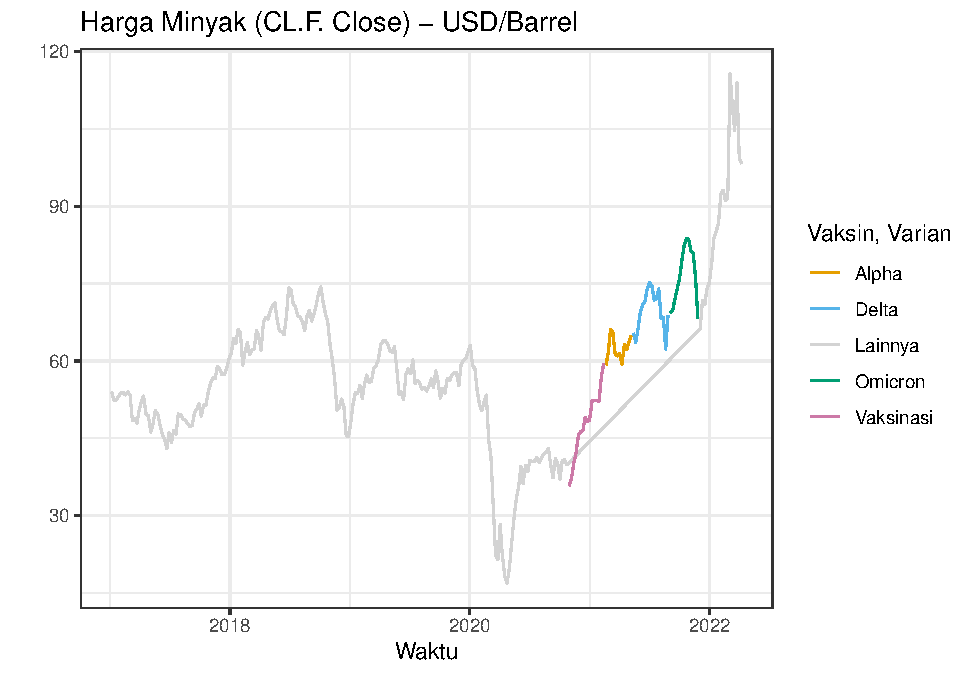
\includegraphics{_main_files/figure-latex/unnamed-chunk-40-1.pdf}

Tren umum harga minyak naik karena optimisme mengenai vaksin. OPEC juga masih membatasi produksi pada awal tahun 2021. Namun, tren tersebut tidak mulus karena muncul beberapa varian COVID-19. Varian Alpha disebut \emph{variant of concern} pada Februari 2021. Harga minyak turun karena infeksi dari varian Alpha meningkat. Lalu, setelah varian tersebut teratasi, pemulihan ekonomi dunia meningkatkan harga minyak. Delta mulai disebut \emph{variant of conern} pada Mei 2021, dan di beberapa negara peningkatan kasus dari Delta masih ada sampai bulan September. Harga minyak turun (\protect\hyperlink{ref-reu_oil_2021}{2021 Agu}). Namun, badai Ida di Amerika Serikat yang mengaggu produksi minyak, penurunan produksi OPEC, dan perbaikan hubungan Amerika Serikat-Tiongkok meningkatkan harga minyak. Saat varian Omicron muncul, harga minyak turun lagi (\protect\hyperlink{ref-resnick-ault_oil_2021}{Resnick-ault 2021 Des}).

\begin{Shaded}
\begin{Highlighting}[]
\NormalTok{cbbPalette2 }\OtherTok{\textless{}{-}} \FunctionTok{c}\NormalTok{(}\StringTok{"\#D3D3D3"}\NormalTok{,}\StringTok{"\#E69F00"}\NormalTok{, }\StringTok{"\#56B4E9"}\NormalTok{)}

\NormalTok{weeklyCrude[,}\StringTok{"2022"}\SpecialCharTok{:}\ErrorTok{=}
              \FunctionTok{ifelse}\NormalTok{(Date}\SpecialCharTok{\textgreater{}=}\FunctionTok{as.Date}\NormalTok{(}\StringTok{"2021{-}12{-}01"}\NormalTok{) }\SpecialCharTok{\&}\NormalTok{ Date}\SpecialCharTok{\textless{}=}\FunctionTok{as.Date}\NormalTok{(}\StringTok{"2022{-}02{-}24"}\NormalTok{),}
                     \StringTok{"Pemulihan Omicron"}\NormalTok{,}
              \FunctionTok{ifelse}\NormalTok{(Date}\SpecialCharTok{\textgreater{}=}\FunctionTok{as.Date}\NormalTok{(}\StringTok{"2022{-}02{-}24"}\NormalTok{),}\StringTok{"Perang Ukraina{-}Russia"}\NormalTok{,}\StringTok{"Lainnya"}\NormalTok{))]}
\FunctionTok{ggplot}\NormalTok{(}\FunctionTok{aes}\NormalTok{(}\AttributeTok{x=}\NormalTok{Date, }\AttributeTok{y=}\NormalTok{Close),}
       \AttributeTok{data=}\NormalTok{weeklyCrude)}\SpecialCharTok{+}
  \FunctionTok{geom\_line}\NormalTok{(}\FunctionTok{aes}\NormalTok{(}\AttributeTok{color=}\StringTok{\textasciigrave{}}\AttributeTok{2022}\StringTok{\textasciigrave{}}\NormalTok{))}\SpecialCharTok{+}\FunctionTok{scale\_color\_manual}\NormalTok{(}\AttributeTok{values=}\NormalTok{cbbPalette2)}\SpecialCharTok{+}
  \FunctionTok{ggtitle}\NormalTok{(}\StringTok{"Harga Minyak (CL.F. Close) {-} USD/Barrel"}\NormalTok{)}\SpecialCharTok{+}\FunctionTok{xlab}\NormalTok{(}\StringTok{"Waktu"}\NormalTok{)}\SpecialCharTok{+}\FunctionTok{ylab}\NormalTok{(}\StringTok{" "}\NormalTok{)}\SpecialCharTok{+}
  \FunctionTok{theme\_bw}\NormalTok{()}
\end{Highlighting}
\end{Shaded}

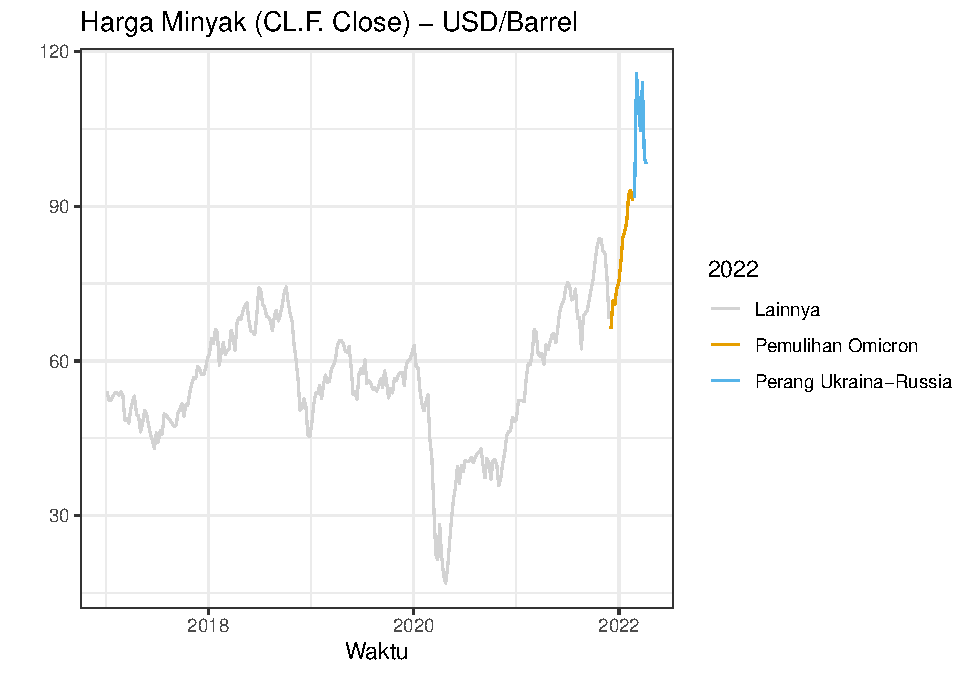
\includegraphics{_main_files/figure-latex/unnamed-chunk-41-1.pdf}

Harga minyak naik di awal tahun 2022 setelah varian Omicron ditemukan memiliki tingkat kematian lebih rendah. Stok minyak di Amerika Serikat menurun, dan stok di Uni Emirat Arab terganggu setelah negara tersebut diserang oleh Houthi. Lalu, perang Rusia-Ukraina pada 24 Februari 2022 meningkatkan harga minyak secara drastis karena impor minyak dari Rusia dapat dihentikan oleh Amerika Serikat dan negara Eropa Barat. Harga minyak turun dari puncaknya di awal Maret setelah Amerika Serikat bernegosiasi dengan Iran dan Venezuela untuk mengganti pasokan minyak, mulai ada perundingan antara Rusia dan Ukraina, serta rencana Amerika Serikat untuk mengeluarkan pasokan strategis minyaknya (\protect\hyperlink{ref-cnn_us_nodate}{Mattingly \emph{et al.} 2022}).

Dampak invasi Rusia ke Ukraina sangat signifikan terhadap harga minyak di negara-negara barat terutama Eropa yang sangat bergantung terhadap minyak dari Rusia. Invasi tersebut menyebabkan disrupsi suplai minyak dari Rusia akibat perang dan rencana embargo minyak mentah karena agresi Rusia mulai diperbincangkan. Harga minyak yang tinggi juga berpengaruh terhadap harga komoditas pangan karena logistik dari satu tempat ke tempat lainnya membutuhkan bahan bakar minyak (\protect\hyperlink{ref-islam_ukraine_nodate}{Islam 2022}).

Selain negara-negara barat, dampak harga minyak juga terasa di negara-negara Asia. Meskipun nilai perdagangan dengan Rusia rendah, kenaikan harga komoditas pangan akibat logistik yang terganggu akan mengakibatkan inflasi semakin parah dan menghambat pemulihan ekonomi pasca pandemi. Untuk mengatasi hal tersebut, berbagai negara seperti Korea dan Jepang memberlakukan subsidi harga minyak untuk meminimalkan dampak ekonomi dari tingginya harga minyak (\protect\hyperlink{ref-kammer_how_nodate}{Kammer \emph{et al.}}).

\hypertarget{pemulusan}{%
\chapter{Pemulusan}\label{pemulusan}}

Under construction!

\hypertarget{pemodelan}{%
\chapter{Pemodelan}\label{pemodelan}}

Under construction!

\hypertarget{refs}{}
\begin{CSLReferences}{0}{0}
\leavevmode\vadjust pre{\hypertarget{ref-barclay_price_2015}{}}%
Barclay MJ, Hendershott T. 2015. Price {Discovery} and {Trading} {After} {Hours}. \emph{The Review of Financial Studies}. 16(4):1041--1073.doi:\href{https://doi.org/10.1093/rfs/hhg030}{10.1093/rfs/hhg030}.

\leavevmode\vadjust pre{\hypertarget{ref-R-ISOweek}{}}%
Block U, Hatto von Hatzfeld using an algorithm by. 2011. \emph{ISOweek: Week of the year and weekday according to ISO 8601}. Ed ke-R package version 0.6-2.

\leavevmode\vadjust pre{\hypertarget{ref-calhoun_saudirussia_nodate}{}}%
Calhoun G. 2020. The {Saudi}/{Russia} {Oil} {Price} {War}: {Historic} {Blunder} \#1. \emph{Forbes}. {[}diunduh 2022 Apr 10{]}. Tersedia pada: \url{https://www.forbes.com/sites/georgecalhoun/2020/06/03/the-other-epidemic-a-cluster-of-historic-blunders---exhibit-1-the-saudirussia-oil-price-war/}

\leavevmode\vadjust pre{\hypertarget{ref-cryer_time_2008}{}}%
Cryer JD, Chan KS. 2008. \emph{Time {Series} {Analysis}: {With} {Applications} in {R}}. Springer New York. (Springer {Texts} in {Statistics}).

\leavevmode\vadjust pre{\hypertarget{ref-dichristopher_us_2018}{}}%
DiChristopher T. 2018 Des. {US} crude tumbles 4.8\% to 17-month low, settling at \$45.88, as stock market slides. \emph{CNBC}. {[}diunduh 2022 Apr 10{]}. Tersedia pada: \url{https://www.cnbc.com/2018/12/20/oil-markets-global-economy-crude-supply-in-focus.html}

\leavevmode\vadjust pre{\hypertarget{ref-R-data.table}{}}%
Dowle M, Srinivasan A. 2021. \emph{data.table: Extension of `data.frame`}. Ed ke-R package version 1.14.2.

\leavevmode\vadjust pre{\hypertarget{ref-fouroil}{}}%
Elshendy M, Colladon AF, Battistoni E, Gloor PA. 2018. Using four different online media sources to forecast the crude oil price. \emph{Journal of Information Science}. 44(3):408--421.doi:\href{https://doi.org/10.1177/0165551517698298}{10.1177/0165551517698298}.

\leavevmode\vadjust pre{\hypertarget{ref-reu_oil_2017-6}{}}%
Gloystein H. 2017 Des. Oil prices near 2015 highs on tight market. \emph{Reuters}. {[}diunduh 2022 Apr 10{]}. Tersedia pada: \url{https://www.reuters.com/article/global-oil-idUSL4N1OS18H}

\leavevmode\vadjust pre{\hypertarget{ref-reu_oil_2017-1}{}}%
Gloystein H. 2017 Jan. Oil prices rise on weakening dollar, but plentiful supplies cap gains. \emph{Reuters}. {[}diunduh 2022 Apr 10{]}. Tersedia pada: \url{https://www.reuters.com/article/global-oil-idUSL4N1FG18Z}

\leavevmode\vadjust pre{\hypertarget{ref-reu_oil_2017-4}{}}%
Gloystein H. 2017 Jun. Oil prices fall on {OPEC} output increase, rising {U}.{S}. crude stocks. \emph{Reuters}. {[}diunduh 2022 Apr 10{]}. Tersedia pada: \url{https://www.reuters.com/article/global-oil-idUSL3N1JB05K}

\leavevmode\vadjust pre{\hypertarget{ref-reu_oil_2018}{}}%
Gloystein H. 2018 Jan. Oil prices drop on uptick in {U}.{S}. production. \emph{Reuters}. {[}diunduh 2022 Apr 10{]}. Tersedia pada: \url{https://www.reuters.com/article/global-oil-idUSL3N1PE14V}

\leavevmode\vadjust pre{\hypertarget{ref-He2018}{}}%
He XJ. 2018. Crude Oil Prices Forecasting: Time Series vs. SVR Models. \emph{Journal of International Technology and Information Management}. 27(2):25--42.

\leavevmode\vadjust pre{\hypertarget{ref-fpp2}{}}%
Hyndman RJ, Athanasopoulos G. 2018. \emph{Forecasting: Principles and Practice}. ed ke-2. Australia: OTexts.

\leavevmode\vadjust pre{\hypertarget{ref-islam_ukraine_nodate}{}}%
Islam F. 2022. Ukraine {Conflict}: {Petrol} at {Fresh} {Record} as {Oil} and {Gas} {Prices} {Soar}. \emph{BBC}. {[}diunduh 2022 Apr 10{]}. Tersedia pada: \url{https://www.bbc.com/news/business-60642786}

\leavevmode\vadjust pre{\hypertarget{ref-kammer_how_nodate}{}}%
Kammer A, Azour J, Selassie AA, Goldfajn I, Rhee C. How {War} in {Ukraine} {Is} {Reverberating} {Across} {World}'s {Regions}. \emph{IMF}. {[}diunduh 2022 Apr 10{]}

\leavevmode\vadjust pre{\hypertarget{ref-khan_economic_2014}{}}%
Khan M. 2014. The {Economic} {Consequences} of the {Arab} {Spring}. \emph{Atlantic Council: Rafik Hariri Center for the Middle East}.:10.

\leavevmode\vadjust pre{\hypertarget{ref-reu_oil_2017}{}}%
Kumar DK. 2017 Jan. Oil falls on {China} concerns, down 3 percent for the week on {OPEC} doubts. \emph{Reuters}. {[}diunduh 2022 Apr 10{]}. Tersedia pada: \url{https://www.reuters.com/article/us-global-oil-idUSKBN14X04K}

\leavevmode\vadjust pre{\hypertarget{ref-reu_oil_2019}{}}%
Kumar DK. 2019 Agu. Oil spills into {U}.{S}.-{China} trade war, prices slump. \emph{Reuters}. {[}diunduh 2022 Apr 10{]}. Tersedia pada: \url{https://www.reuters.com/article/us-usa-trade-china-oil-idUSKCN1VD22D}

\leavevmode\vadjust pre{\hypertarget{ref-tlioil}{}}%
Li T. 2021. The 2008 Financial Crisis and Its Effects on Gas and Oil. \emph{Investopedia}. {[}diunduh 2022 Apr 7{]}. Tersedia pada: \url{https://www.investopedia.com/ask/answers/052715/how-did-financial-crisis-affect-oil-and-gas-sector.asp}

\leavevmode\vadjust pre{\hypertarget{ref-cnn_us_nodate}{}}%
Mattingly P, Liptak K, Collins K, Egan M. 2022. {US} and allies agree to release 60 million barrels of oil from their reserves as {Russian} invasion of {Ukraine} causes price spike - {CNNPolitics}. {[}diunduh 2022 Apr 10{]}. Tersedia pada: \url{https://edition.cnn.com/2022/03/01/politics/us-strategic-petroleum-reserve-release-latest/index.html}

\leavevmode\vadjust pre{\hypertarget{ref-mead_2014_2015}{}}%
Mead D, Stiger P. 2015. The 2014 plunge in import petroleum prices: {What} happened? \emph{Beyond the Numbers: Global Economy}. 4(9).

\leavevmode\vadjust pre{\hypertarget{ref-lw_oil_2020}{}}%
Mills A. 2020 Apr. Oil {ETFs}, {Contango} and negative oil prices. \emph{Livewire Markets}. {[}diunduh 2022 Apr 10{]}. Tersedia pada: \url{https://www.livewiremarkets.com/wires/oil-etfs-contango-and-negative-oil-prices}

\leavevmode\vadjust pre{\hypertarget{ref-R-imputeTS}{}}%
Moritz S, Gatscha S. 2021. \emph{imputeTS: Time Series Missing Value Imputation}. Ed ke-R package version 3.2.

\leavevmode\vadjust pre{\hypertarget{ref-reu_oil_2021}{}}%
Oil prices fall on {U}.{S}. crude stock build, {Delta} variant spread. 2021 Agu. \emph{CNBC}. {[}diunduh 2022 Apr 10{]}. Tersedia pada: \url{https://www.cnbc.com/2021/08/04/oil-markets-covid-delta-variant.html}

\leavevmode\vadjust pre{\hypertarget{ref-pfizer_2020}{}}%
Pfizer. 2020 Nov. Pfizer and {BioNTech} {Announce} {Vaccine} {Candidate} {Against} {COVID}-19 {Achieved} {Success} in {First} {Interim} {Analysis} from {Phase} 3 {Study}. \emph{Business Wire}. {[}diunduh 2022 Apr 10{]}. Tersedia pada: \url{https://www.businesswire.com/news/home/20201109005539/en/\%C2\%A0Pfizer-and-BioNTech-Announce-Vaccine-Candidate-Against-COVID-19-Achieved-Success-in-First-Interim-Analysis-from-Phase-3-Study}

\leavevmode\vadjust pre{\hypertarget{ref-voxoil}{}}%
Plumer B. 2014. Oil prices keep plummeting as {OPEC} starts a price war with the {US}. \emph{Vox}. {[}diunduh 2022 Apr 7{]}. Tersedia pada: \url{https://www.vox.com/2014/11/28/7302827/oil-prices-opec}

\leavevmode\vadjust pre{\hypertarget{ref-resnick-ault_oil_2021}{}}%
Resnick-ault J. 2021 Des. Oil prices post weekly loss on {Omicron} uncertainty. \emph{Reuters}. {[}diunduh 2022 Apr 10{]}. Tersedia pada: \url{https://www.reuters.com/markets/commodities/oil-heads-flat-week-omicron-uncertainty-2021-12-17/}

\leavevmode\vadjust pre{\hypertarget{ref-R-quantmod}{}}%
Ryan JA, Ulrich JM. 2020. \emph{quantmod: Quantitative Financial Modelling Framework}. Ed ke-R package version 0.4.18.

\leavevmode\vadjust pre{\hypertarget{ref-soverflow}{}}%
Stefan (https://stackoverflow.com/users/1494637/stefan). 2019. converting daily stock data to weekly-based via pandas in Python. \emph{Stack Overflow}.

\leavevmode\vadjust pre{\hypertarget{ref-welle_wwwdwcom_us_nodate}{}}%
{US} to end sanctions waivers for {Iranian} oil imports {\textbackslash{}}textbar {DW} {\textbackslash{}}textbar 22.04.2019. 2019. \emph{Deutsche Welle}. {[}diunduh 2022 Apr 10{]}. Tersedia pada: \url{https://www.dw.com/en/us-to-end-sanctions-waivers-for-iranian-oil-imports/a-48435237}

\leavevmode\vadjust pre{\hypertarget{ref-guardoil}{}}%
Wearden G. 2009. Oil price creeps back towards 100 a barrel. \emph{The Guardian}. {[}diunduh 2022 Apr 7{]}. Tersedia pada: \url{https://www.theguardian.com/business/2009/jun/10/oil-price-increase}

\leavevmode\vadjust pre{\hypertarget{ref-R-ggplot2}{}}%
Wickham H, Chang W, Henry L, Pedersen TL, Takahashi K, Wilke C, Woo K, Yutani H, Dunnington D. 2021. \emph{ggplot2: Create Elegant Data Visualisations Using the Grammar of Graphics}. Ed ke-R package version 3.3.5.

\leavevmode\vadjust pre{\hypertarget{ref-R-dplyr}{}}%
Wickham H, François R, Henry L, Müller K. 2022. \emph{dplyr: A Grammar of Data Manipulation}. Ed ke-R package version 1.0.8.

\leavevmode\vadjust pre{\hypertarget{ref-woolich_sanctions_nodate}{}}%
Woolich A, Martin D, Hunt S, Arroyo P. 2018. Sanctions {Update}: {US} sanctions on {Iran}, 8 {May} 2018. \emph{Holman Fenwick Willan}. {[}diunduh 2022 Apr 10{]}. Tersedia pada: \url{https://www.hfw.com/Sanctions-Update-US-sanctions-on-Iran-8-May-2018}

\leavevmode\vadjust pre{\hypertarget{ref-R-timeDate}{}}%
Wuertz D, Setz T, Chalabi Y, Maechler M, Byers JW. 2018. \emph{timeDate: Rmetrics - Chronological and Calendar Objects}. Ed ke-R package version 3043.102.

\leavevmode\vadjust pre{\hypertarget{ref-R-strucchange}{}}%
Zeileis A, Leisch F, Hornik K, Kleiber C. 2019. \emph{strucchange: Testing, Monitoring, and Dating Structural Changes}. Ed ke-R package version 1.5-2.

\end{CSLReferences}

\end{document}
